% mnras_template.tex 
%
% LaTeX template for creating an MNRAS paper
%
% v3.0 released 14 May 2015
% (version numbers match those of mnras.cls)
%
% Copyright (C) Royal Astronomical Society 2015
% Authors:
% Keith T. Smith (Royal Astronomical Society)

% Change log
%
% v3.0 May 2015
%    Renamed to match the new package name
%    Version number matches mnras.cls
%    A few minor tweaks to wording
% v1.0 September 2013
%    Beta testing only - never publicly released
%    First version: a simple (ish) template for creating an MNRAS paper

%%%%%%%%%%%%%%%%%%%%%%%%%%%%%%%%%%%%%%%%%%%%%%%%%%
% Basic setup. Most papers should leave these options alone.
\documentclass[fleqn,usenatbib]{mnras}

% MNRAS is set in Times font. If you don't have this installed (most LaTeX
% installations will be fine) or prefer the old Computer Modern fonts, comment
% out the following line
\usepackage{newtxtext,newtxmath}
% Depending on your LaTeX fonts installation, you might get better results with one of these        :
%\usepackage{mathptmx}
%\usepackage{txfonts}

% Use vector fonts, so it zooms properly in on-screen viewing software
% Don't change these lines unless you know what you are doing
\usepackage[T1]{fontenc}
\usepackage{ae,aecompl}


%%%%% AUTHORS - PLACE YOUR OWN PACKAGES HERE %%%%%

% Only include extra packages if you really need them. Common packages are:
\usepackage{graphicx}	% Including figure files
\usepackage{amsmath}	% Advanced maths commands
\usepackage{amssymb}	% Extra maths symbols

%%%%%%%%%%%%%%%%%%%%%%%%%%%%%%%%%%%%%%%%%%%%%%%%%%

%%%%% AUTHORS - PLACE YOUR OWN COMMANDS HERE %%%%%

% Please keep new commands to a minimum, and use \newcommand not \def to avoid
% overwriting existing commands. Example:
%\newcommand{\pcm}{\,cm$^{-2}$}	% per cm-squared
\newcommand{\red}[1]{{\textcolor{red}{#1}}}
\newcommand{\green}[1]{{\textcolor{green}{#1}}}
\newcommand{\blue}[1]{{\textcolor{blue}{#1}}}

%%%%%%%%%%%%%%%%%%%%%%%%%%%%%%%%%%%%%%%%%%%%%%%%%%

%%%%%%%%%%%%%%%%%%% TITLE PAGE %%%%%%%%%%%%%%%%%%%

% Title of the paper, and the short title which is used in the headers.
% Keep the title short and informative.
\title[Origin of kinematic misalignment]{SDSS-IV MaNGA: Kinematic misalignment in about 6000 galaxies: revealing the evolutionary pathways leading to offsets between stellar and gas rotation}

% The list of authors, and the short list which is used in the headers.
% If you need two or more lines of authors, add an extra line using \newauthor
\author[C. Duckworth et al.]{Christopher Duckworth,$^{1}$\thanks{E-mail: cd201@st-andrews.ac.uk}
Rita Tojeiro,$^{1}$
Third Author$^{2,3}$
and Fourth Author$^{3}$
\\
% List of institutions
{}$^{1}$School of Physics and Astronomy, University of St Andrews, North Haugh, St Andrews, KY16 9SS, UK\\
$^{2}$Department, Institution, Street Address, City Postal Code, Country\\
$^{3}$Another Department, Different Institution, Street Address, City Postal Code, Country
}

% These dates will be filled out by the publisher
\date{Accepted XXX. Received YYY; in original form ZZZ}

% Enter the current year, for the copyright statements etc.
\pubyear{2019}

% Don't change these lines
\begin{document}
\label{firstpage}
\pagerange{\pageref{firstpage}--\pageref{lastpage}}
\maketitle

% Abstract of the paper
\begin{abstract}
We use $\sim$ 4000 galaxies from the MaNGA IFU survey to investigate the morphological dependence of the decoupling of rotation between stars and gas. We find this, that and this.

The factors leading to the decoupling of star and gas rotation are diverse and are strongly dependent on morphology (probably). We create a mock MaNGA observational sample in the cosmological scale hydrodynamical simulation IllustrisTNG to investigate the assembly history and driving factors of misalignment. We find this, that and those.

Talk about potential use for misalignment to be additional proxy in finding lower angular momentum haloes.
\end{abstract}

% Select between one and six entries from the list of approved keywords.
% Don't make up new ones.
\begin{keywords}
keyword1 -- keyword2 -- keyword3
\end{keywords}
\section{Introduction}
\red{Make factors of little h explicit throughout the document}
\section{Data}
\subsection{The MaNGA survey}
Set to complete in 2020, the MaNGA survey is designed to investigate the internal structure of $\sim$10000 galaxies in the nearby Universe. By design, the complete sample is unbiased towards morphology, inclination and colour and provides a near flat distribution in stellar mass. 

MaNGA is one of three programs in the fourth generation of the Sloan Digital Sky Survey (SDSS-IV) which enables detailed kinematics through integral field unit (IFU) spectroscopy. MaNGA uses the SDSS 2.5 meter telescope in spectroscopic mode \citep{gunn2006} with the two dual-channel BOSS spectrographs \citep{smee2013} and the MaNGA IFUs \citep{drory2015}. MaNGA provides spatial resolution on kpc scales (2'' diameter fibres) while covering 3600-10300$\mathring{A}$ in wavelength with a resolving power that varies from R$\sim$1400 at 4000$\mathring{A}$ to R$\sim$2600 at 9000$\mathring{A}$. 

MaNGA observations are covered plate by plate, employing a dithered pattern for each galaxy corresponding to one of the 17 fibre-bundles of 5 distinct sizes. \red{Describe the sizes here?} Any incomplete data release of MaNGA should therefore be unbiased with respect to IFU sizes and hence a reasonable representation of the final sample scheduled to be complete in 2020.

The majority of observations contribute to one of the three main subsets: the Primary sample, the Secondary sample and the Colour-Enhanced supplement. All sub-samples observe galaxies to a minimum of $\sim 1.5$ effective radii ($R_{e}$) with the Secondary sample increasing this minimum to $\sim 2.5 R_{e}$. The Colour-Enhanced supplement fills in gaps of the colour-magnitude diagram leading to an approximately flat distribution of stellar mass. A full description of the MaNGA observing strategy is given in \citet{law2015obs,yan2016obs}. 
The raw observations are processed by the MaNGA Data 
Reduction Pipeline (DRP) as described in \citet{law2016drp, yan2016spec}. The fibre flux and inverse variance is extracted from each exposure, which are then wavelength calibrated, flat-fielded and sky subtracted. In this work, we use 6044 galaxies from the eighth MaNGA Product Launch (MPL-8) that are selected in the Primary, Secondary and Colour-Enhanced samples and have non-critical observations. Figure \ref{fig:samp_cons} shows the distribution of stellar mass and redshift of the eighth MaNGA Product Launch (MPL-8) with comparison to the NASA-Sloan Atlas (NSA) catalogue from which MaNGA is targeted and our $\Delta$PA defined sub-sample outlined in \S\ref{sec:samp_sec}.

\begin{figure}
	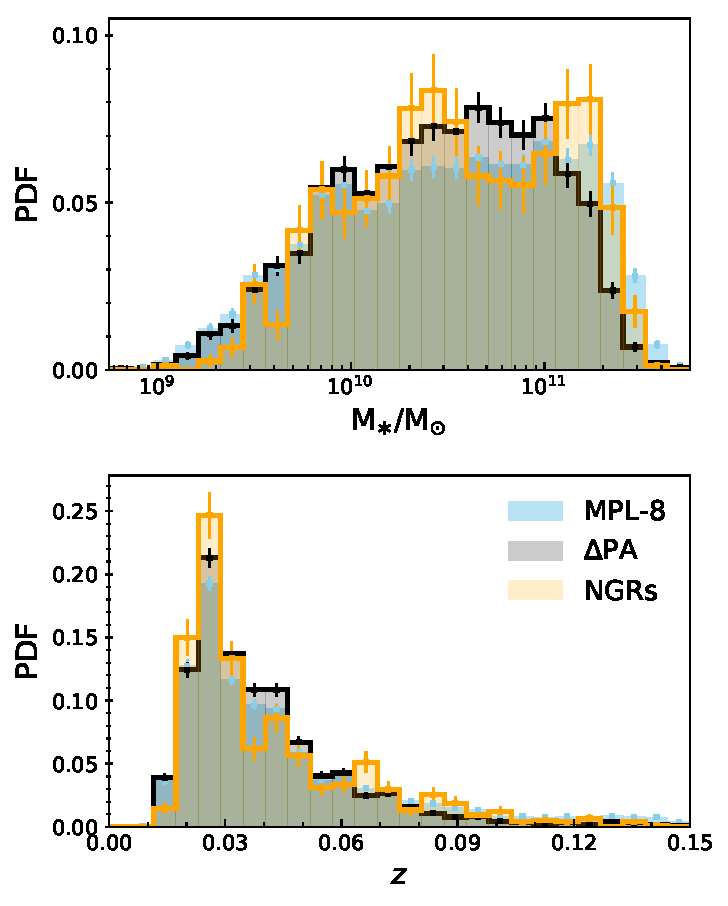
\includegraphics[width=\linewidth]{total_pop/mpl8_pa_stelmass_z.pdf}
    \caption{Relative frequency distributions of stellar mass and redshift for the NSA target catalogue (brown dotted line), MaNGA MPL-8 (gray dashed line), our $\Delta$PA sub-sample (black solid line) and those with a defined stellar PA but no clear H$\alpha$ rotation (green dot-dashed line). The figure is cut at $z=0.15$ representing the extent of MaNGA targets. Each histogram is given with Poisson errors on each bin.}
    \label{fig:samp_cons}
\end{figure}

\subsection{Spectral fitting for kinematics}
All stellar and H$\alpha$ velocity fields are taken directly from the MaNGA Data Analysis Pipeline \citep[DAP;][for an overview and emission line modelling respectively]{westfall2019, belfoire2019}, we direct the reader to these references, however we summarise the key points here.

The DAP extracts stellar kinematics using the Penalised Pixel-Fitting (pPXF) method \citep{cappellari2004,cappellari2017}. The DAP fits the stellar continuum of each spaxel to extract the line of sight velocity dispersion and then fits the absorption-line spectra from a set of 49 clusters of stellar spectra from the MILES stellar library \citep{sanchez2006,falcon2011}. Before extraction of the mean stellar velocity, the spectra are spatially Voronoi binned to $g$-band \textit{S/N} $\sim$ 10, excluding any individual spectrum with a $g$-band \textit{S/N} < 1 \citep{cappellari2003}. This approach is geared towards stellar kinematics as the spatial binning is applied to the continuum \textit{S/N}, however, we note that unbinned and Voronoi binned velocity maps produce similar results. 

Ionized gas kinematics are extracted by the DAP through fitting a Gaussian to the H$\alpha$-6564 emission line, relative to the input redshift for the galaxy. This velocity is representative for all ionized gas, since the parameters for each Gaussian fit to each emission line are tied during the fitting process. These velocities are also binned spatially by the Voronoi bins of the stellar continuum. 

\subsection{Defining global position angles}
For a complete description of PA fitting and typical error estimation for MaNGA, we direct the reader to Duckworth+19. Here we use a similar process, summarising the key points and highlighting differences with respect to Duckworth+19.

Global position angles (PA) are estimated for both the stellar and ionized gas velocity fields using the \texttt{fit\_kinematic\_pa} routine \citep[see Appendix C of][for a description of the process]{krajnovic2006}. \texttt{fit\_kinematic\_pa} returns the angle (counter-clockwise) of the bisecting line which has greatest velocity change along it. The best fit angle is found by sampling 181 equally spaced steps, so that the output PA will have precision of 0.5$^{\circ}$. By default, \texttt{fit\_kinematic\_pa} returns a PA defined between 0$^{\circ}$ and 180$^{\circ}$, which is indiscriminate towards direction of the blueshifted and redshifted sides. To adjust this, we identify the redshifted side and return PAs defined by the angle to the redshifted side clockwise from the north axis (0-360$^{\circ}$). 

The accuracy of PA fitting is biased by neighbouring galaxies, spectral pixels (spaxels) with spuriously high velocities and inclination. 

Foreground stars are removed during the spectral fitting, however foreground/background galaxies can remain within the IFU footprint. This can be a significant problem for global PA fitting since \texttt{fit\_kinematic\_pa} symmetrizes the velocity fields and interpolates to estimate the PA. Background/small objects can then bias the PA fit for the main target, especially in the instance where they are moving significantly different to the target galaxy. To counteract this, we remove all disconnected regions smaller than $10\%$ of the target galaxy's footprint. 

Spaxels with spuriously high velocities (e.g. > 1000km/s relative to target's central redshift) can also bias PA fits during symmetrization. These often correspond to background galaxies that are connected (on the sky) to the target galaxy's footprint, and hence, we sigma clip the velocity field and remove all spaxels above a $3\sigma$ threshold.

Accurate PA estimation is naturally more difficult for near edge-on galaxies. \green{Obscuration - talk to AM/Rita} and a smaller surface area allow individual Voronoi bins to more easily bias overall PA fits. This inherently leads to a larger scatter in PA fitting around the true value, especially due to central spaxels during symmetrization.

\subsection{Visual Classifications}
Global position angles are only well defined for coherently rotating velocity fields. Those with a decoupling between inner and outer regions due to warps or kinematically decoupled cores are poorly described by global PAs. 

To select a clean sample of galaxies with well defined global PAs, we visually classify all of the velocity fields after pre-processing and PA fitting. Both stellar and H$\alpha$ velocity fields are characterised into 3 categories;
\begin{itemize}
    \item Dominant coherent rotation and well defined PA
    \item Dominant coherent rotation but with higher noise or more complex motion resulting in a usable PA fit but with higher typical errors. Highly inclined velocity fields with high likelihood of biased PAs fits are included in this category. 
    \item Do not use.
\end{itemize}

Kinematic features are also identified. Both stellar and H$\alpha$ velocity fields are classified into;
\begin{itemize}
    \item Kinematically decoupled core
    \item Warp (velocity field of central region is warped with respect to outskirts)
    \item Merger (ongoing merger or neighbour within IFU)
    \item No feature
\end{itemize}
The majority of those with kinematic features have poorly defined global PAs and hence are flagged as do not use for the previous flag. \green{Eyeball the field for all MaNGA galaxies.}. 

For studies of quenching it may be useful to consider galaxies that have defined stellar rotation but lack coherent motion in the ionized gas. For galaxies that have usable PAs for the stellar velocity but unusable PAs for the ionized gas, we define a further classification of the gas velocity field;
\begin{itemize}
    \item Depletion (seen as empty spaxels signifying lack of gas, usually central)
    \item No clear rotation (map has no clear rotation or is noise dominated)
    \item Biased rotation (partial rotation in the velocity field, however there are significant regions with incoherent motion)
    \item No clear characteristics/ None.
\end{itemize}
We note there is a clear overlap between the classifications for depletion and no clear rotation, since velocity fields are often a combination of these two features. The total numbers for each classification in each category are summarised in Table \ref{tab:kin_class}. Examples of PA fits (see \S\ref{sec:def_kin_mis} for calculation) with the associated photometry for various kinematic classifications is given in Figure \ref{fig:mis_grid}. Examples of galaxies that are kinematically aligned, misaligned, have a stellar KDC, have a warped H$\alpha$ velocity field and have clear stellar rotation but depleted ionized gas/ no rotation are shown respectively. 

\begin{table*}
\begin{tabular}{lrrrrrrlll}
\hline
&  Clean PA &  Messy PA &  Unusable PA &  KDC &  Warp &  Merger & Depletion & No clear rotation & Biased rotation \\
\hline
Stellar &      3290 &      1581 &         1172 &   47 &    39 &     116 &       960 &               960 &             960 \\
H$\alpha$ &      2876 &      1071 &         2097 &   17 &    82 &     116 &       562 &               180 &             175 \\
Both &      2848 &      1023 &         1136 &    5 &    11 &     116 &        -- &                -- &              -- \\
\end{tabular}
\caption{Summary table of galaxy numbers for kinematic classifications in  MPL-8. Total numbers are defined for stellar (H$\alpha$) velocity fields solely and for both meeting the criteria. Columns 1-3 correspond to the quality of the PA fit, 4-6 correspond to kinematic features and 7-9 correspond to additional notes for the H$\alpha$ velocity field (see text for details about classifications). Columns 7-9 are only defined for unusable PAs for H$\alpha$ and clean/messy PAs for the stellar field. The total number of galaxies meeting this criteria is given in the stellar row for columns 7-9.}
\label{tab:kin_class}
\end{table*}

\begin{figure*}
	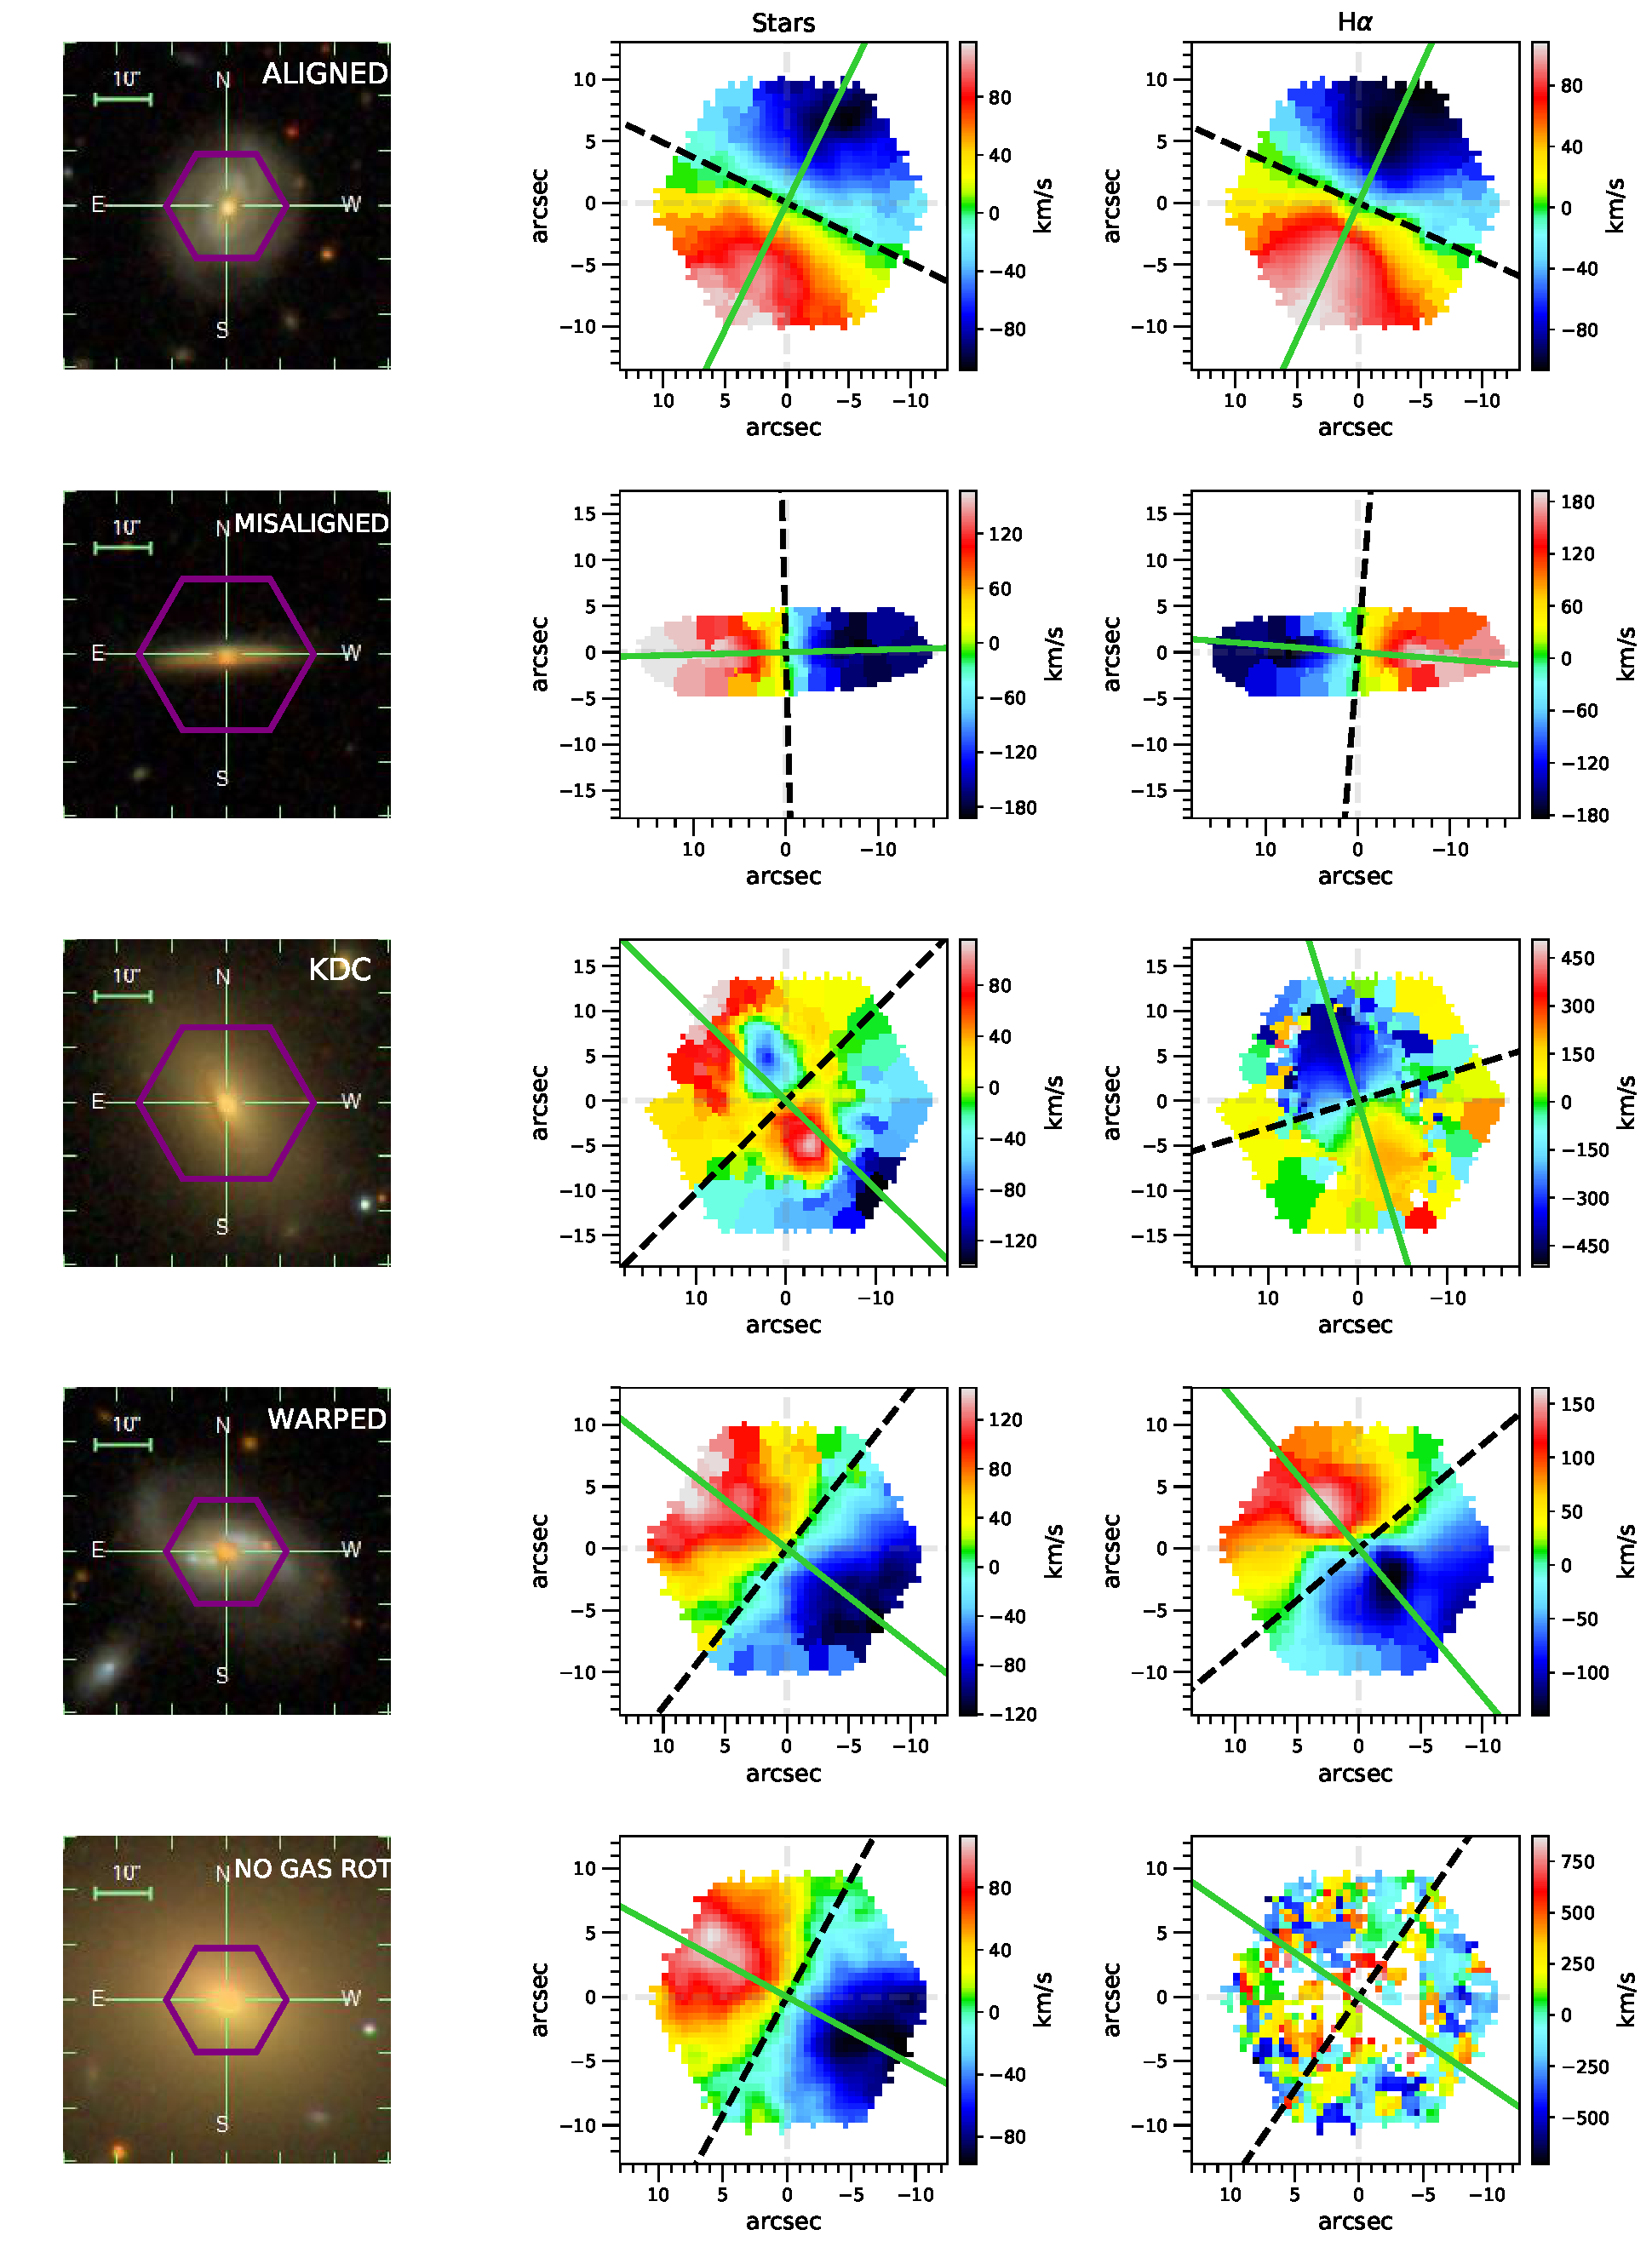
\includegraphics[width=0.8\linewidth]{misalignment_grid.pdf}
    \caption{Examples of PA fits for galaxies with different kinematic classifications. For each galaxy (row), we show the photometry taken from SDSS with the MaNGA IFU observation footprint overlaid in purple, the stellar velocity field and the H$\alpha$ velocity field. The kinematic PA fits (see \S\ref{sec:def_kin_mis}) are shown on the velocity fields (green solid line) with the axis of rotation (black dotted line). The kinematic classifications from top to bottom are; (a) PLATEIFU: 7958-6101, kinematically aligned near face on; (b) PLATEIFU: 8465-12704, counter-rotating near edge on; (c) PLATEIFU: 9868-12704, with a KDC in the stellar velocity; (d) PLATEIFU: 8252-6103, with a warped H$\alpha$ velocity field with respect to the stellar; (e) PLATEIFU: 10219-6102, with a centrally depleted/missing H$\alpha$ velocity field but coherent rotation in the stellar.}
    \label{fig:mis_grid}
\end{figure*}

\subsection{Defining kinematic misalignment} \label{sec:def_kin_mis}
Only selecting galaxies with dominant coherent rotation (both clean and messy) for both stellar and H$\alpha$ velocity fields with no defined features in either map, we are left with 3798 galaxies used in this analysis. The mass distribution of the $\Delta$PA defined sample with respect to MPL-8 is shown in Figure \ref{fig:samp_cons}. For the purpose of quantifying external interaction, we define the offset angle between the kinematic PAs of the stellar and ionized gas fields as such; 
\begin{equation} \label{eq:delPA}
\Delta PA = |PA_{stellar} - PA_{H\alpha}|. 
\end{equation}
We define galaxies with $\Delta$PA > 30$^{\circ}$ to be significantly kinematically misaligned. \green{why?}

\subsection{Morphology} \label{sec:morph_def}
We classify the morphology of $\Delta$PA defined MaNGA galaxies through the formalism laid out by the citizen science project; GalaxyZoo2 \citep[GZ2;][]{willett2013}. GZ2 provides visually identified morphologies (and also measures finer morphological features e.g. bars, bulge size and edge-on disks) for 304,122 galaxies drawn from SDSS. GZ2, however, is not complete for the MaNGA sample and has been combined with an unpublished version; GalaxyZoo4 with debiasing code re-run to provide a consistent set of definitions for all MaNGA targets (see; \url{https://www.sdss.org/dr15/data_access/value-added-catalogs/?vac_id=manga-morphologies-from-galaxy-zoo}). 

In a nutshell, GZ2 provides morphological classification through a decision tree of questions. Further questions are dependent on the answer to the previous to characterise a certain morphological type and identify finer features (see Figure 1 in \citep{willett2013} for this flowchart). From this, a table of vote fractions for each question combined with the total number of votes dictate a reliably sampled galaxy population with a set of desired morphological features. 

The first question in the decision tree 'Is the galaxy smooth and rounded with no sign of a disk?', allows categorisation into broad Early type (ETGs) and Late type galaxies (LTGs). We select galaxies with a debiased vote fraction > 0.7 for smooth to be ETGs and galaxies with a debiased vote fraction of > 0.7 for disk or features to be LTGs. \green{Should remove features?}. Defining an exact population of lenticular galaxies (S0s) is tricky through public classifications. LTGs, however, can be separated based on the dominance of the bulge with respect to the disk in GZ2 through the question 'How prominent is the central bulge, compared with the rest of the galaxy?'. \citep{willett2013} demonstrate a strong correlation between bulge dominance as defined per this question and expert classifications of T-type \citep{nair2010}. Equation 19 of \citet{willett2013} provides a linear mapping from GZ2 bulge classification to expert defined morphological T-type. Care must be taken in using this linear mapping \citep[see discussion in][]{willett2013}, however, this should be a reasonable parameterisation to coarsly separate LTGs into earlier-type (S0 - Sa) and later-type spirals (Sb - Sd). We split our LTG population at T-type = 3, to give three morphological categories along with pure ETGs. \green{Table with numbers of galaxies for each category.}

\subsection{Group membership and halo mass definitions} \label{sec:group_def}
To investigate different pathways leading to kinematic misalignment, we must separate galaxies into centrals and satellites and consider the size of the group that they reside in. 

We identify groups with an adaptive halo-based group finder of \citet{yang2005,yang2007} and with improved halo mass assigning techniques \citep[see;][for details and application to SDSS]{lim2017}. In a nutshell, the group finder uses either the stellar mass or luminosity of central galaxies in addition with the nth brightest/most massive satellite as proxies for halo mass. Galaxies are assigned to groups through an iterative process, where halo properties such as halo size and velocity dispersion are updated until membership converges. For groups that are outside of the redshift limit where groups are complete \green{$\sim 0.7$ for SDSS?}, final halo masses are assigned through abundance matching. Those incomplete are assigned halo masses based on the ranking between halo mass and the proxy found at the final iteration of the group finder.

The performance of the group finder has been tested on realistic mock catalogues, showing that the halo masses of individual haloes are consistent with the true mass with a typical scatter of $\sim$0.2 dex. This scatter is similar to the commonly used group finder of \citet{yang2007}, however extends uniformly to halo masses 0.7 dex lower. 

For this work, we use the stellar mass based halo mass proxy for the SDSS main sample. \citet{lim2017} do not apply the group finder to the thin strips in the Southern Galatic Cap of SDSS main due to incomplete groups resulting from close proximity to borders. MaNGA galaxies in these strips are therefore unclassified by the group finder, resulting in 5088 matched galaxies with halo mass estimates and group membership classifications into central or satellite.

% \subsection{Pipe3D}
% We use spatially resolved derived properties, such as SFR gradients, gas mass, $\lambda_{R}$... using the Pipe3D pipeline. or maybe we dont. \citep{pipe3Da,pipe3Dvac}.

\subsection{IllustrisTNG}
The IllustrisTNG project \citep{marinacci18,naiman18,nelson18,pillepich18b,springel18} is a suite of magneto-hydrodynamic cosmological scale simulations incorporating an updated comprehensive model for galaxy formation physics \citep[as decribed in; ][]{weinberger17,pillepich18a} and making use of the moving-mesh code \texttt{AREPO} \citep{springel10,pakmor11,pakmor13}. For this work, we use the highest resolution fiducial run of TNG-100 (hereafter referred to as TNG) which follows the evolution of 2 x 1820$^3$ resolution elements within a periodic cube with box lengths of 110.7 Mpc (75 h$^{-1}$ Mpc). This corresponds to an average mass resolution of baryonic elements of 1.4 x 10$^6 M_{\odot}$ and 7.5 x 10$^6 M_{\odot}$ for dark matter. 

Structure in TNG is identified into haloes and subhaloes as follows. Haloes (also referred to as FoF haloes or Groups) are found from a standard friends-of-friends (FoF) algorithm \citep{davis85} with linking length b=0.2. The FoF algorithm is run on the dark matter particles, and the other types (gas, stars, BHs) are attached to the same groups as their nearest DM particle. Each halo is then divided into gravitationally bound subhaloes through the subfind algorithm \citep{springel01}.

We consider all subhaloes at $z=0$ (snapshot 99) containing a minimum stellar mass of $M_{\ast} = 10^{8} M_{\odot}$ that are gravitationally bound to the subhalo (as defined by subfind), to potentially make up our mock MaNGA like sample. 

\subsubsection{Matching to MaNGA sample}
To construct a mock MaNGA sample we select representative subhaloes from TNG. For every MaNGA galaxy, we find the subhalo with the most similar stellar mass, effective light radius and $g - r$ colour \red{SDSS like - describe other matches and weighting}. The subhalo is then assigned the same size IFU as the matched MaNGA galaxy with the corresponding angular resolution. The subhalo is then `observed' at a distance so that the angular footprint of the assigned IFU covers the same number of physical effective radii for the mock galaxy as the matched observation. 

\red{Statement about inclination}
\red{rewrite this} Matching on these parameters ensures that the mock sample is consistent with MaNGA to first order and enables comparison for the overall populations. \red{annalisa's paper? demonstrates that the overall TNG galaxy population deviates from real galaxies in these ways... so differences are expected even in the case of perfect matching}. 

\subsubsection{Mock observations}
We convert each subhalo in TNG into a mock MaNGA observation, as follows:

We take the raw particle data of gas and stars and project on the XY plane (i.e. z-direction is the line of sight). Since there is no preferred direction in the simulation, this corresponds to a 'random' viewing angle of each galaxy (although talk about matching on inclination). We bin particles corresponding to the angular resolution of spaxels in MaNGA (0.5 arcsec/pixel), in the distinct hexagonal fibre bundle footprint. In each bin, we calculate the mean velocity, velocity dispersion and total flux for all particles.

Since we include all particles along the line of sight, we must take care in interpreting the absolute values of flux, since none is lost due to obscuration. We, however, only use the flux values relatively when calculating the luminosity weighted averages of velocity and dispersion while estimating $\lambda_R$. 

In order to estimate the typical noise associated with a MaNGA observation, we compute radial profiles of the signal to noise ratio (SNR) for all MaNGA observations of a given IFU fibre bundle size. MaNGA provides estimates of the SNR for every spaxel in each observation in the g-band. Figure \ref{fig:noise_profile} shows the azimuthally averaged SNR profiles for all MaNGA observations of each fibre bundle size. We fit a logarithmic function to each profile, which is used to assign noise to the mock observations. Noise is drawn for each pixel from a normal distribution using the median and standard deviation of the fitted logarithmic radial profile.   

\begin{figure}
	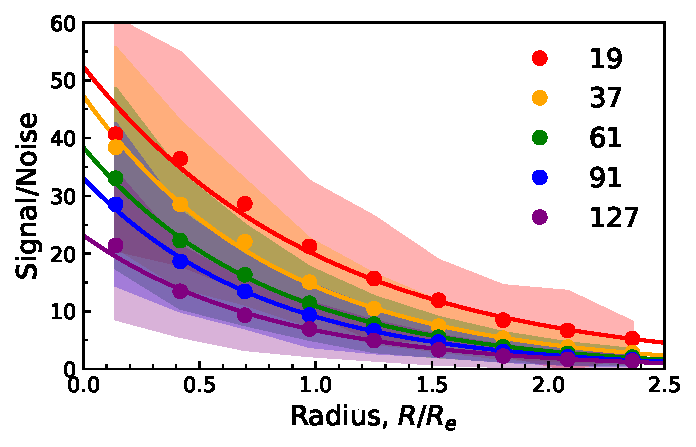
\includegraphics[width=\linewidth]{noise_profiles_ifusize.pdf}
    \caption{Average signal to noise profiles for each IFU size for all MaNGA MPL-8 observations. The circles show the median value for each radius bin with the shaded region corresponding to the standard deviation. The solid line corresponds to an logarithmic parametric fit to the data points, used in sampling the noise profile for the mock observations.}
    \label{fig:noise_profile}
\end{figure}

In order to simulate the effects of the point spread function (PSF), we then convolve our binned particle data with a Gaussian kernel. MaNGA observations typically have a g-band PSF which can be fit with a Gaussian of $\sim 2-3''$ full width half maximum (FWHM). We take all our mock observations to have a PSF modelled by a Gaussian with a 2$''$ FWHM. 

We fit position angles to MaNGA observations that have been voronoi bins containing a minimum S/N $\sim 10$. To maintain consistency and avoid spurious individual particles biasing measurements, we also voronoi bin our mock observations so that a minimum of 5 particles is contained within a given bin. Figure \ref{fig:example_obs} shows example stellar (and gas) velocity and dispersion fields along with normalised r-band flux, after our processing. 

\begin{figure*}
	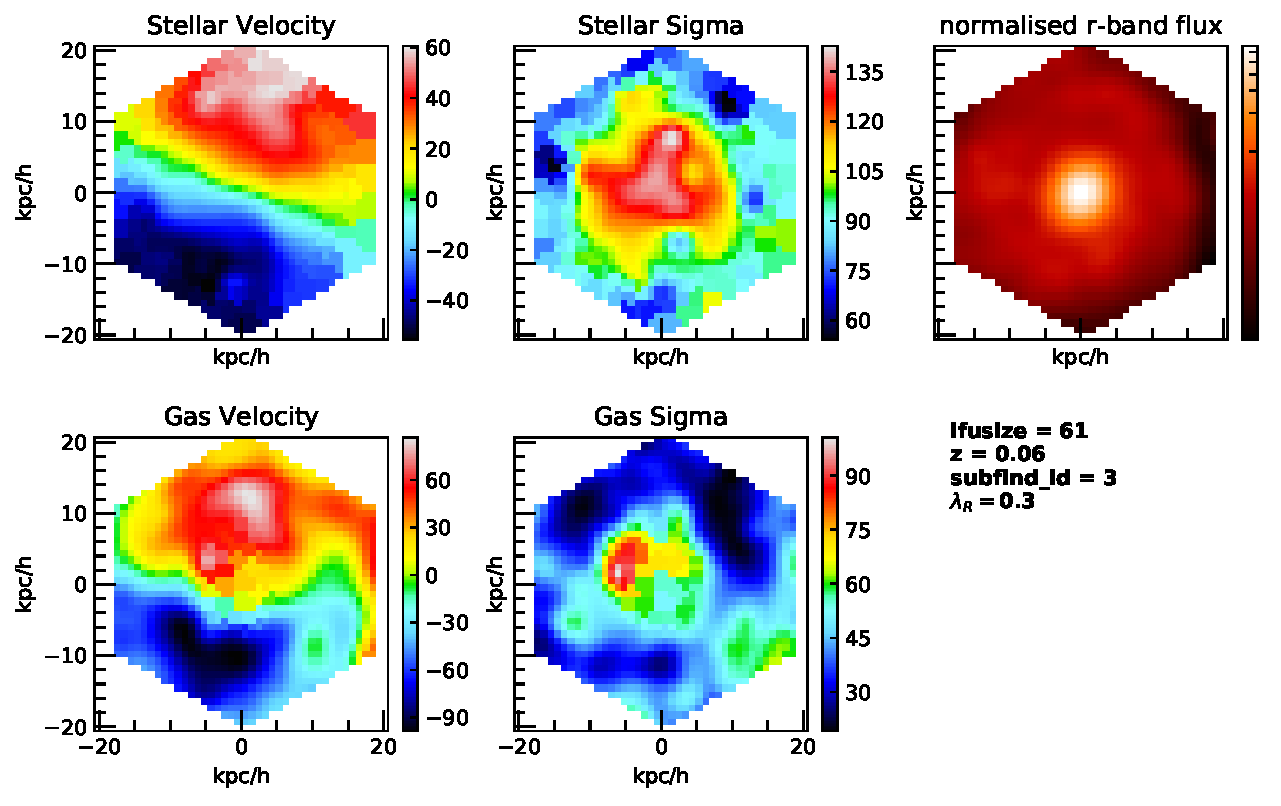
\includegraphics[width=\linewidth]{example_grid.pdf}
    \caption{Output MaNGA-like maps for an example TNG subhalo. Top row: Stellar velocity field, stellar dispersion field and normalised r-band flux (in logarithmic scale; arbitrary units). Bottom row: gas velocity and dispersion fields.}
    \label{fig:example_obs}
\end{figure*}

\section{Results}
\subsection{Total population} \label{sec:manga_total_pop}
Firstly we consider all $\Delta$PA defined galaxies (i.e. selecting all stellar and H$\alpha$ velocity fields with clean or messy defined PAs) for MaNGA \red{and for our matched comparison sample in IllustrisTNG}. Figure \ref{fig:total_pa_dist}, shows the distribution of $\Delta$PA for MaNGA and IllustrisTNG. \red{Discussion about comparison between MaNGA and TNG}

\begin{figure}
	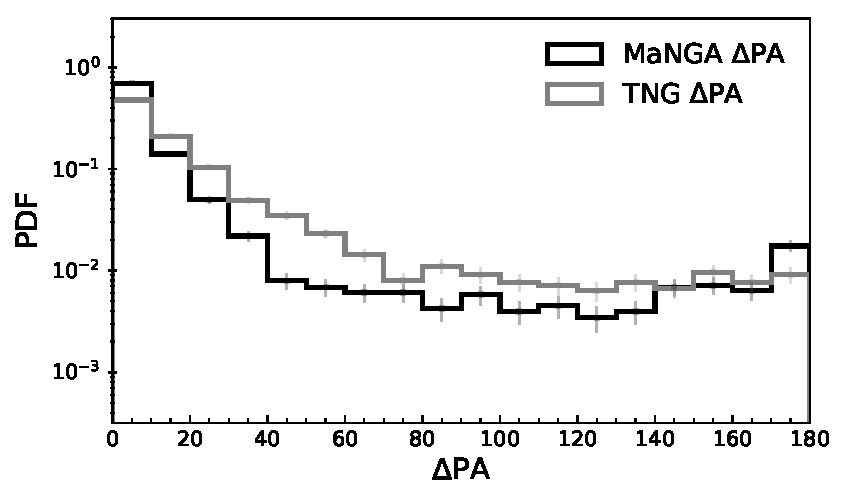
\includegraphics[width=\linewidth]{total_pop/mpl8_pa_dist.pdf}
    \caption{Probability density distribution of kinematic misalignment as defined by $\Delta$PA for the total MaNGA sample (black solid line) \red{and matched TNG-100 sample.} $\Delta$PA is strongly peaked around 0$^{\circ}$ with a small boost close to 180$^{\circ}$.}
    \label{fig:total_pa_dist}
\end{figure}

We now divide our MaNGA $\Delta$PA defined population at $\Delta$PA = 30$^{\circ}$ into aligned and misaligned (see \S\ref{sec:def_kin_mis} for choice of 30$^{\circ}$ reasoning). In the following, we also consider galaxies with defined stellar PAs but undefined H$\alpha$ due to central depletion or incoherent rotation/dispersion domination (NGRs). Figure \ref{fig:delPA_stelM} shows the distribution of stellar mass for these three populations. Kinematically aligned and misaligned galaxies appear to be consistent in stellar mass, whereas NGRs appear to be preferentially more massive. \citet{graham2018} previously demonstrated the tight correlation between stellar angular momentum and stellar mass for MaNGA (MPL-5; $\sim$2300 galaxies). Since NGRs are typically higher mass, it could be expected that they are less rotationally supported with respect to the $\Delta$PA defined populations. Figure \ref{fig:delPA_lambda_Re}, shows $\lambda_R$ vs $\epsilon$ for all $\Delta$PA defined galaxies and the medians for the aligned, misaligned and NGR samples. Kinematically aligned galaxies reside at preferentially higher $\lambda_R$ and ellipticity with respect to NGRs. This is indicative of the dispersion dominance over rotation for disrupted gas poor and typically higher mass galaxies that we see in our NGR sample. Interestingly, kinematically misaligned galaxies also typically reside close to the slow rotator regime (defined by the black solid line). This suggests that NGRs and kinematically misaligned galaxies have had similar levels of disruption to their angular momentum, most likely due to interactions and mergers, in their recent history. \red{NGRs more massive and hence would naturally expect them to reside closer to slow rotator regime in comparison to misaligned galaxies. Expand on this discussion.}

\begin{figure}
	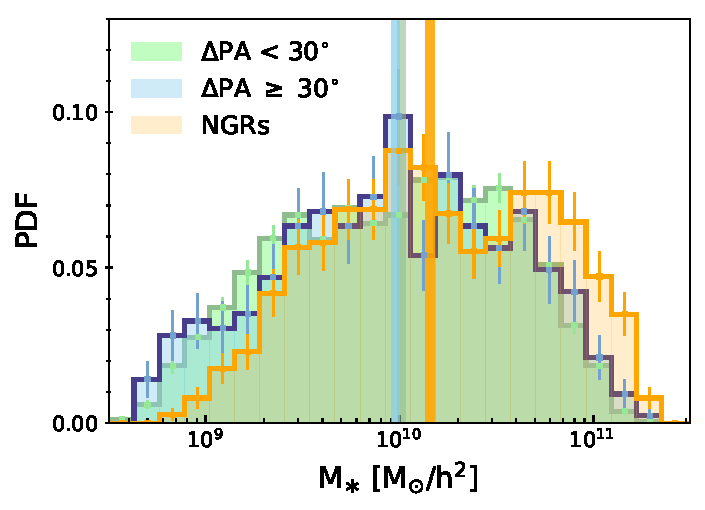
\includegraphics[width=\linewidth]{total_pop/delPA_stelM.pdf}
    \caption{Probability density distributions of stellar mass, $(M_{\ast}/M_{\odot})$ for aligned galaxies ($\Delta$PA < 30$^{\circ}$) shown with black (solid line), those with high misalignment ($\Delta$PA > 30$^{\circ}$) are in red (solid line) and NGRs are in green (dot-dashed line). Each histogram is given with Poisson errors on each bin. The vertical lines denote the corresponding distribution's median. Splitting on $\Delta$PA shows no marked difference in stellar mass, however, those without gas rotation are preferentially more massive.}
    \label{fig:delPA_stelM}
\end{figure}

\begin{figure*}
	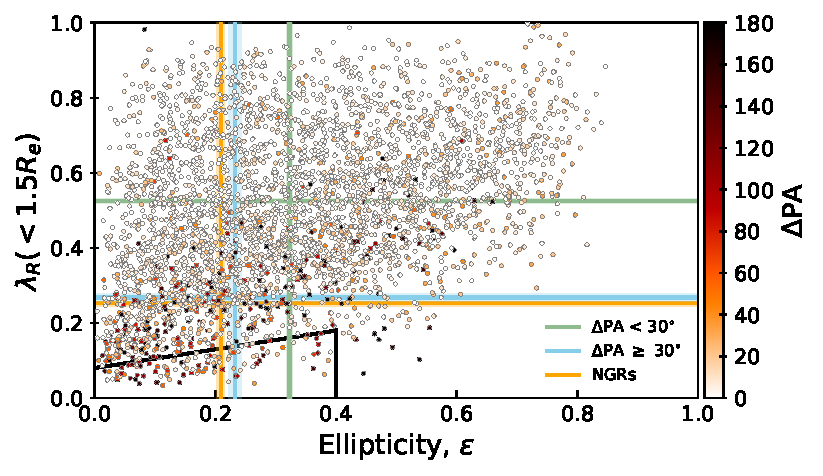
\includegraphics[width=\linewidth]{total_pop/delPA_lambda_Re.pdf}
    \caption{$\lambda_R$ within 1.5$R_e$ against ellipticity, $\epsilon$ for all galaxies with defined $\Delta$PA. Medians for kinematically aligned ($\Delta$PA < 30$^{\circ}$), misaligned ($\Delta$PA > 30$^{\circ}$) and NGR are shown by the black, red and green dashed lines respectively. Aligned galaxies reside more typically in the fast rotator regime with higher $\lambda_R$ and $\epsilon$, whereas misaligned galaxies and NGRs reside closer to the slow rotator regime.}
    \label{fig:delPA_lambda_Re}
\end{figure*}

\subsection{Morphology}
We now sub-divide the total population by morphology into ETGs, S0/Sas and Sb/Sds as defined in \S\ref{sec:morph_def}. Figure \ref{fig:morph_PA}, shows the distributions for each category. We find that for all morphological types, galaxies are most commonly aligned with strong peaks below $\Delta$PA $\sim 30^{\circ}$. ETGs show a flatter distribution than their later counterparts, as the most likely to exhibit misalignment. LTGs show deeper drop-offs above $\Delta$PA $\sim 40^{\circ}$, with a boost around $\Delta$PA = 180$^{\circ}$, seen most strongly for the Sb/Sds. We quantify the overall misalignment fractions in the first column of Table \ref{tab:mega_table}. This morphological difference in misalignment is likely a result of several factors. Gas rich LTGs have typically higher specific angular momentum, and hence, require a higher magnitude gas inflow to create an offset in rotation. Conversely, ETGs are more dispersion dominated and gas poor enabling smaller gas in-flows (or outflows) to create a kinematic misalignment. 

These misalignment fractions of ETGs are roughly consistent with previous findings in \red{ATLAS3D} and for LTGs similar to those found in \red{SAMI}. 

\red{The boost in the PDF around 180$^{\circ}$ suggests that near counter-rotation is a stable state for galaxies. This is seen most prominently in Sb/Sds. A possible explanation is that these rotation dominated galaxies host strong stellar torques, which act to realign gas on much faster timescales than in ETGs. Counter-rotators, however, remain stable and hence contribute proportionally higher to the misaligned distribution, as those at intermediate misalignments settle towards alignment. Stellar torques act to realign disrupted gas on the order of $\sim X$ dynamical timescales. Check $\lambda_{R}$ for counter-rots - are they lower ang mom due to significant disruption?!} Interestingly, galaxies that exhibit near-counter rotation ($\Delta$PA $\geq$ 150$^{\circ}$) have similar angular momentum to the general misaligned population ($\Delta$PA $\geq$ 30$^{\circ}$), significantly lower than the aligned counterparts. \red{This is indicative of the previous disruption that the galaxies experienced...}

\begin{figure}
	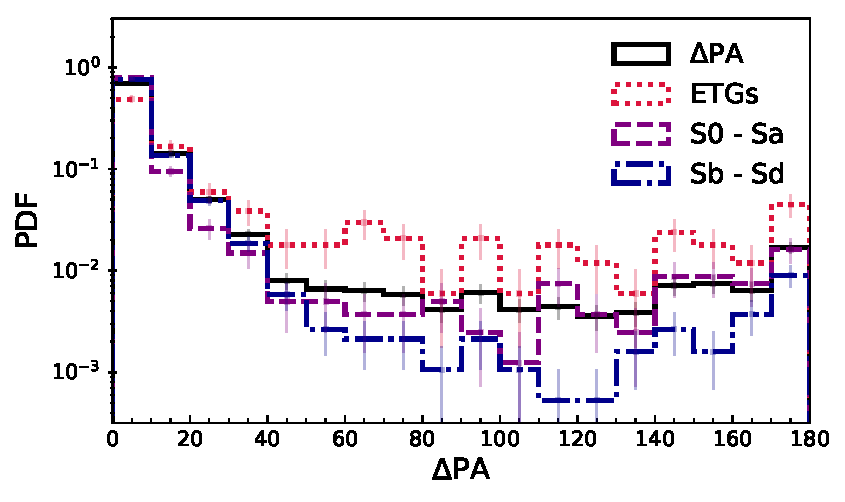
\includegraphics[width=\linewidth]{morph/delPA_morph.pdf}
    \caption{Probability density distributions of kinematic misalignment as defined by $\Delta$PA split on morphology. Distributions for the total population, ETGs, S0/Sa and Sb/Sds are shown by black solid, dotted red, dashed purple and dot-dashed blue lines respectively. Earlier type galaxies are more likely to be misaligned than later type galaxies. red{Add near counter-rotators to median lines.}}
    \label{fig:morph_PA}
\end{figure}

Due to the tight relationship between stellar mass, morphology and specific angular momentum \citep[e.g. see;]{cortese2016}, it would be expected that misaligned galaxies should be at higher stellar mass due to their lower $\lambda_{R}$ with respect to the aligned. Surprisingly for the overall population we see no difference, however, splitting on morphology as shown in Figure \ref{fig:morph_stelM} reveals individual trends. Misaligned ETGs (and NGRs) are more massive than the aligned counterparts most likely indicative of the richer recent merger history for these samples. 

The opposite trends are seen for both S0/Sas and Sb/Sds with kinematically aligned galaxies being of typically higher mass than the misaligned. \red{Simply due to mergers still but losing material to larger neighbour rather than gaining it like ETGs? To explain: why are aligned S0s so massive.} 

\begin{figure}
	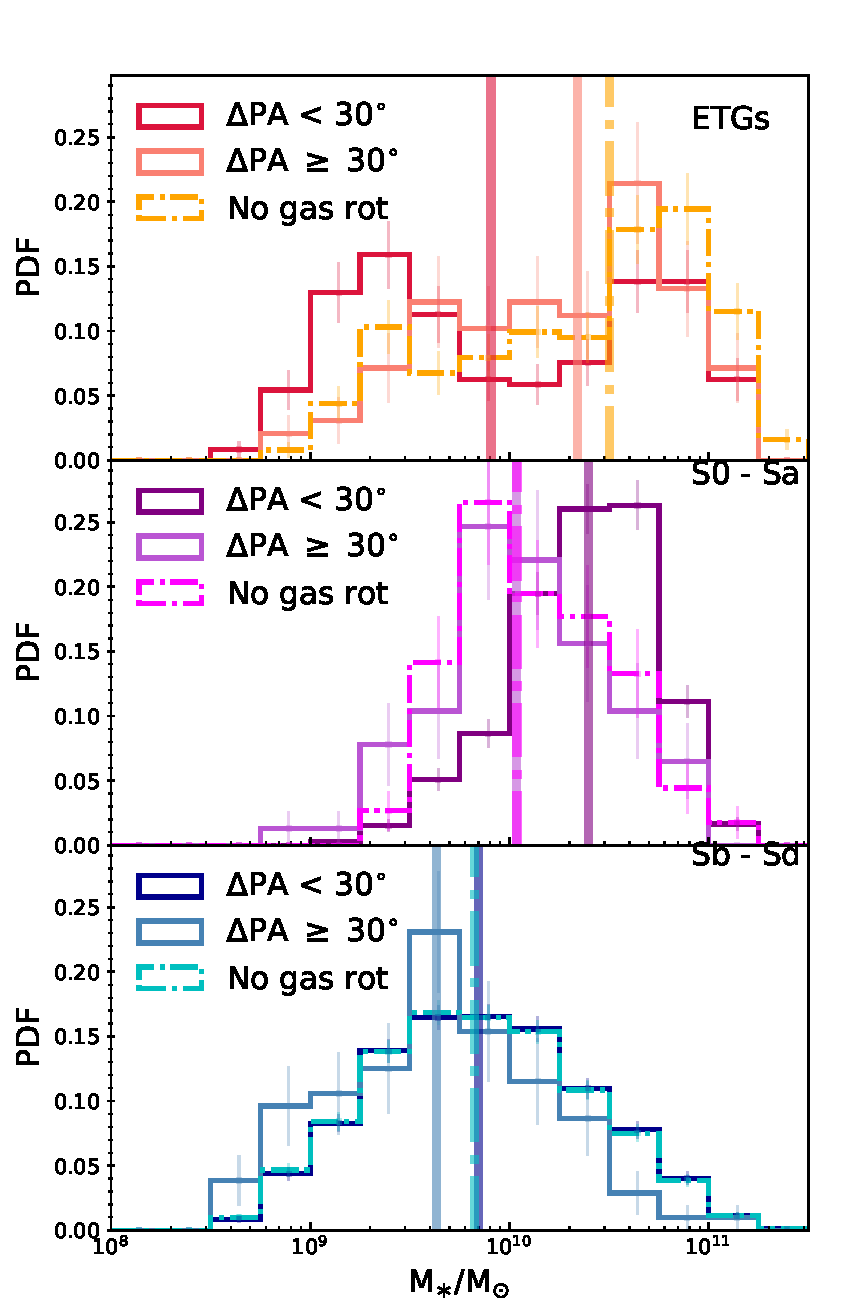
\includegraphics[width=\linewidth]{morph/delPA_stelM_morph.pdf}
    \caption{Probability density distributions of stellar mass, $(M_{\ast}/M_{\odot})$ for aligned galaxies ($\Delta$PA < 30$^{\circ}$, misaligned galaxies ($\Delta$PA > 30$^{\circ}$) and NGRs for ETGs, S0/Sas and Sb/Sds (top to bottom). In each panel the aligned/misaligned are shown with solid lines with the aligned in the darker shade. NGRS are shown by dot-dashed lines. Each histogram is given with Poisson errors on each bin. The vertical lines denote the corresponding distribution's median. For ETGs, aligned galaxies are less massive than the misaligned sample. This trend, however, reverses for S0/Sas and Sb/Sds.}
    \label{fig:morph_stelM}
\end{figure}

\subsection{Group membership}
Group membership is important for dictating the evolution of a galaxy and hence we now sub-divide our population in centrals and satellites as described in \S\ref{sec:group_def}. Figure \ref{fig:group_morph_PA} shows the $\Delta$PA distributions as before, but now split into centrals and satellites. Qualitatively there is no noticeable difference, however Table \ref{tab:mega_table} reveals that centrals are more likely to be misaligned than satellites for ETGs. \red{Add to Table: numbers of NGRs.} Additionally we see that NGRs are far more likely to be satellites for all morphologies. This is indicative that the gas poor NGRs are a population undergoing quenching, \red{typically in more massive groups - add figure showing halo masses for populations?}

\begin{figure*}
	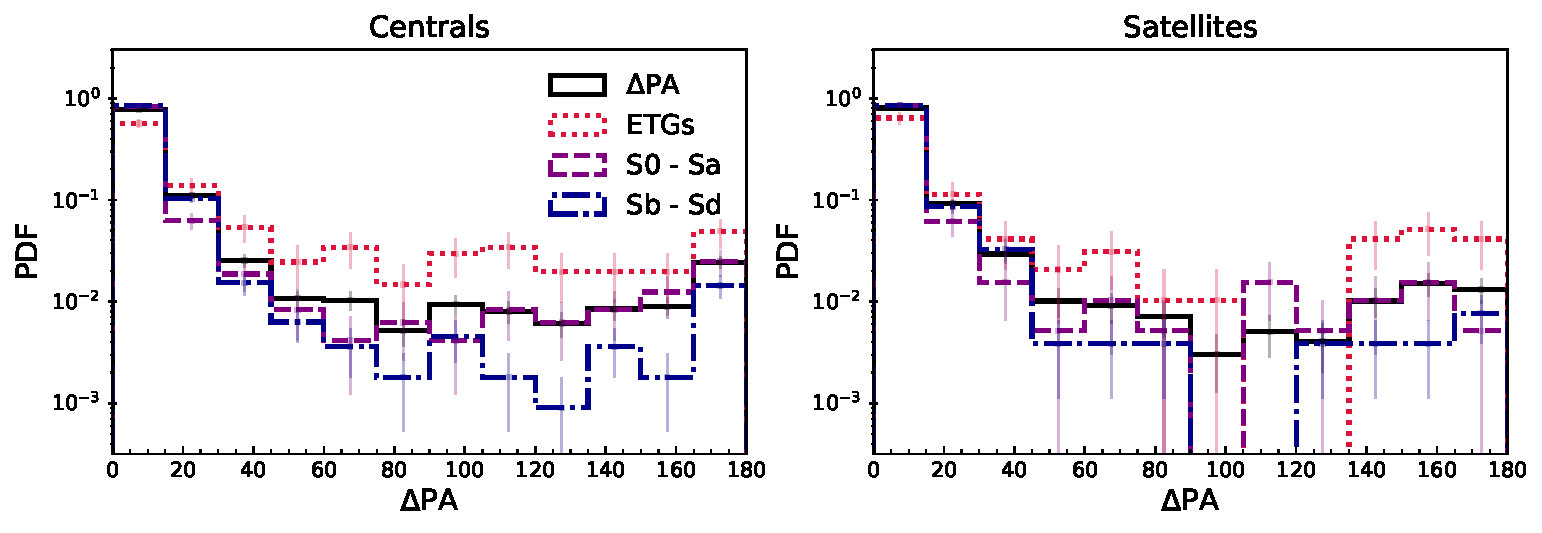
\includegraphics[width=\linewidth]{cen_sat/delPA_morph_lim.pdf}
    \caption{Same as Figure \ref{fig:morph_PA}, however split by group membership into centrals (left) and satellites (right).}
    \label{fig:group_morph_PA}
\end{figure*}

\begin{table}
\begin{tabular}{llll}
\hline
          &           All &      Centrals &    Satellites \\
\hline
      All &  11.1\% (3798) &  11.5\% (2185) &  10.1\% (1007) \\
     ETGs &   27.9\% (301) &   29.4\% (204) \red{[140]} & 24.7\% (97) \red{[91]} \\
 S0 - Sas &    9.7\% (677) &   10.1\% (483) \red{[44]} &    8.8\% (194) \red{[56]} \\
 Sb - Sds &   5.4\% (1634) &   5.2\% (1112) \red{[32]} & 5.7\% (522) \red{[75]} \\
\end{tabular}
\caption{Percentages of galaxies kinematically misaligned ($\Delta$PA $\geq 30^{\circ}$) for all galaxies, centrals and satellites (left to right). Each row shows the percentage for different morphologies with the total number of $\Delta$PA defined galaxies in each cell given in curly brackets. The total number NGRs for a given category is given in the square brackets.}
\label{tab:mega_table}
\end{table}


\begin{figure*}
	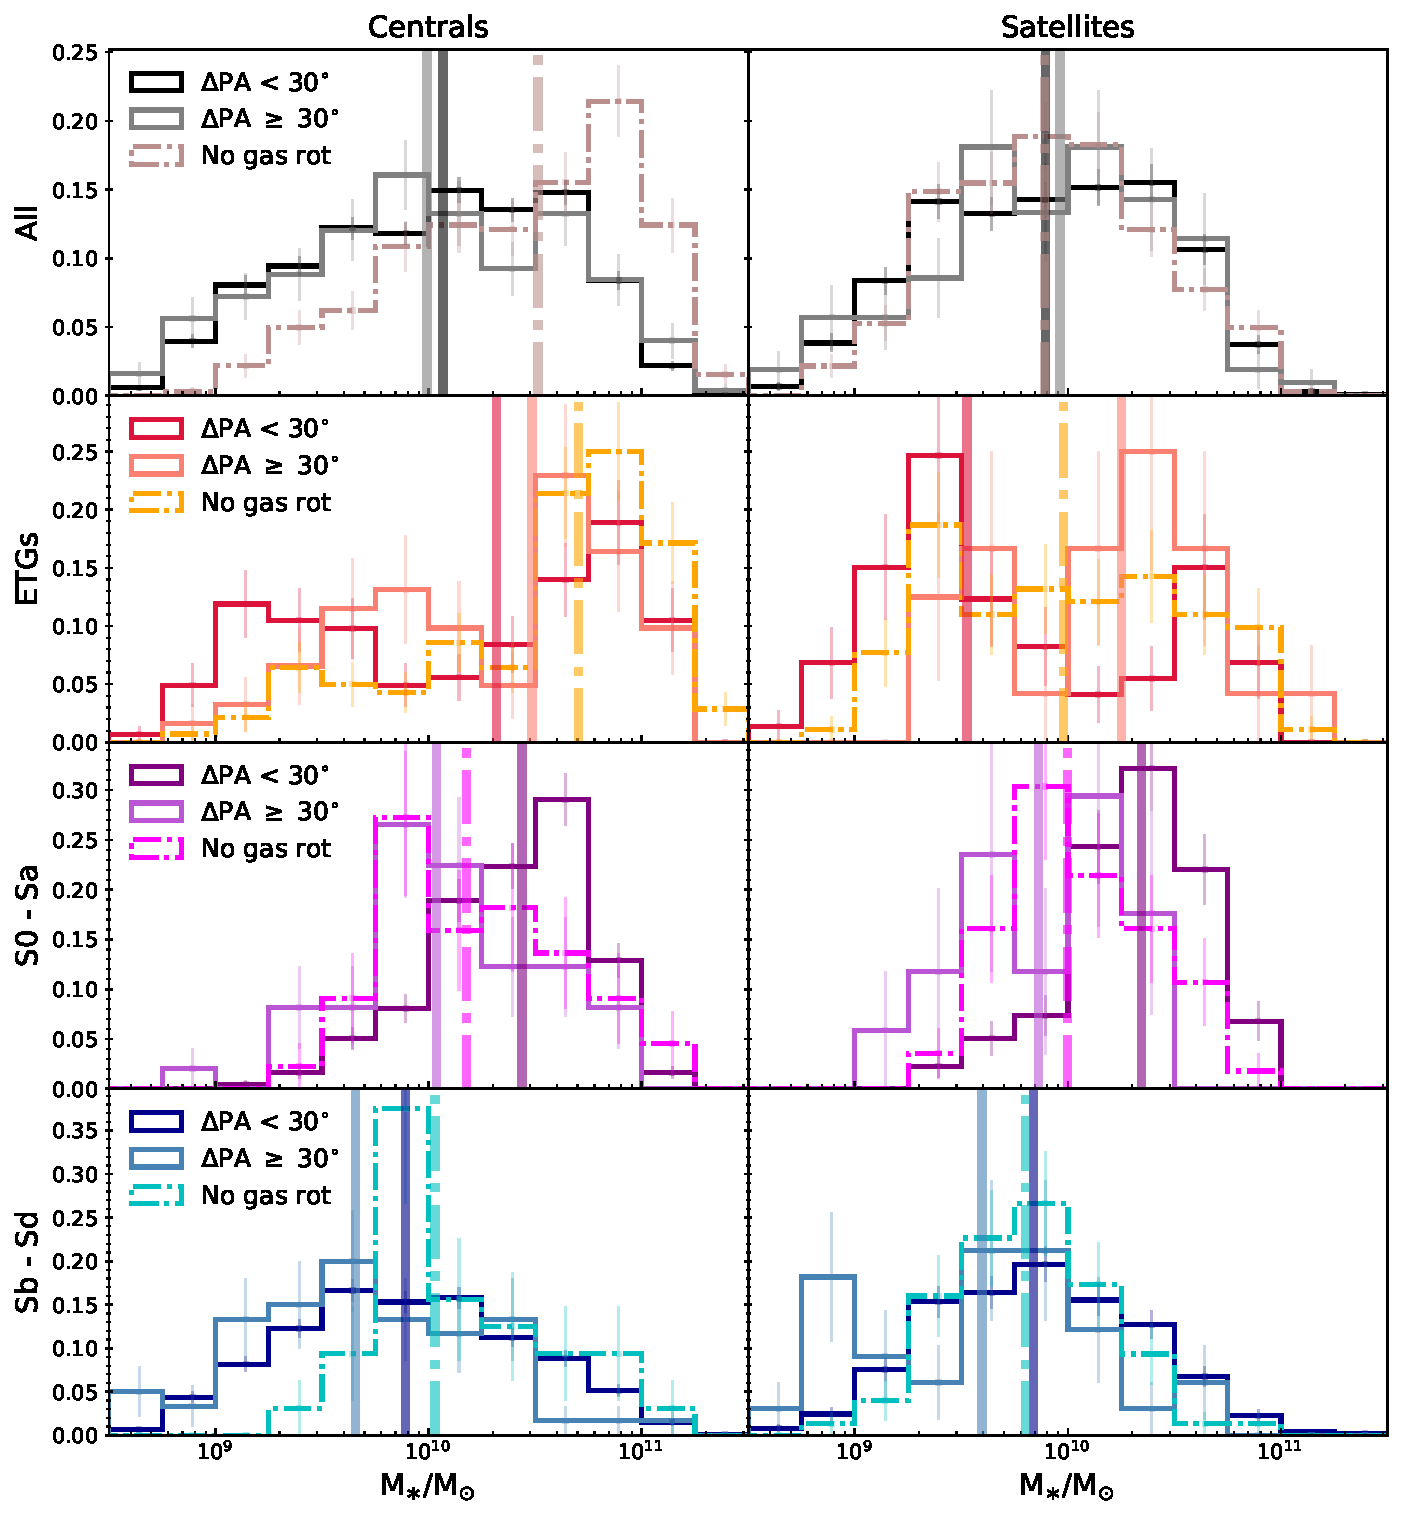
\includegraphics[width=\linewidth]{cen_sat/delPA_stelM_morph_lim.pdf}
    \caption{Same as Figure \ref{fig:morph_stelM}, however split by group membership into centrals (left) and satellites (right). Additionally the distributions for the overall central and satellite populations is shown in the top row. We see that for ETGs there is a strong difference in mass between aligned and misaligned satellites. This trend is reversed for S0/Sa and Sb/Sd satellites. These trends are also seen for centrals, however, typically to a lesser degree.}
    \label{fig:group_morph_stelM}
\end{figure*}

\section{Properties of misaligned galaxies in TNG}
In this section, we utilise the mock sample created in TNG to interpret the properties of kinematically misaligned galaxies in MaNGA and isolate the driving mechanisms. 

\red{discuss inability to use individual matchings to describe sample - point out difficulties with TNG galaxy sample?}. 
We define the morphology of the mock MaNGA sample based on the instantaneous star formation rate within twice the stellar half mass radius of a given galaxy with respect to all other subhalos in TNG. The star forming main sequence for all subhalos is found iteratively by fitting a power law as a function of mass. A galaxy is then flagged into one of three categories; star forming, green valley or quenched depending on its deviation above or below the main sequence \citep{pillepich2019}. This split reproduces the qualitative trends of misalignment probability and morphology (see Appendix \ref{sec:mock_appendix} for more detail). In the following subsections, we follow the evolutionary history of the mock sample split on this morphology definition. 

\subsection{Angular momentum}
In this sub-section, we consider the angular momentum content of our TNG mock sample back to $z=1$ for stars, gas and dark matter individually. Angular momentum for our TNG galaxies is defined by the intrinsic specific angular momentum of their particles
\begin{equation}
J_{k} = \frac{1}{\sum_{n} m^{(n)}} \sum_{n} m^{(n)}\boldsymbol{x}^{(n)} \times \boldsymbol{v}^{(n)}
\end{equation}
where $\boldsymbol{v}^{(n)}$ is the velocity of each particle relative to the centre of mass for the subhalo. $\boldsymbol{x}^{(n)}$ is the position of a given particle with respect to the position of the most gravitationally bound particle in the subhalo. We choose this definition since the centre of mass velocity can be biased by structure at large radii and hence may spuriously not represent the true rotational centre. $k$ is the particle/cell type referring to either stars, gas or dark matter. For stars and gas this is calculated within the 3D radius equivalent to sky coverage assigned by the mock IFU observation. Dark matter is calculated for all particles assigned to the subhalo by the subfind algorithm. 

Figure \ref{fig:sJ_evo} shows the specific angular momentum evolution from $z=1$ for all components split on group membership and morphology. We see that similar to the observational sample (see \S\ref{sec:manga_total_pop}), misaligned galaxies in observations are significantly lower angular momentum than their aligned counterparts at $z=0$ for the stellar components. This is reflected in all components (stars, gas, DM) to various degrees for all morphologies and central/satellite definition. Interestingly, while misalignment between stars and gas may itself be a transient property, those misaligned at $z = 0$ reside in dark matter haloes with \textit{fundamentally lower angular momentum} which persists past $z = 1$. 

\begin{figure*}
	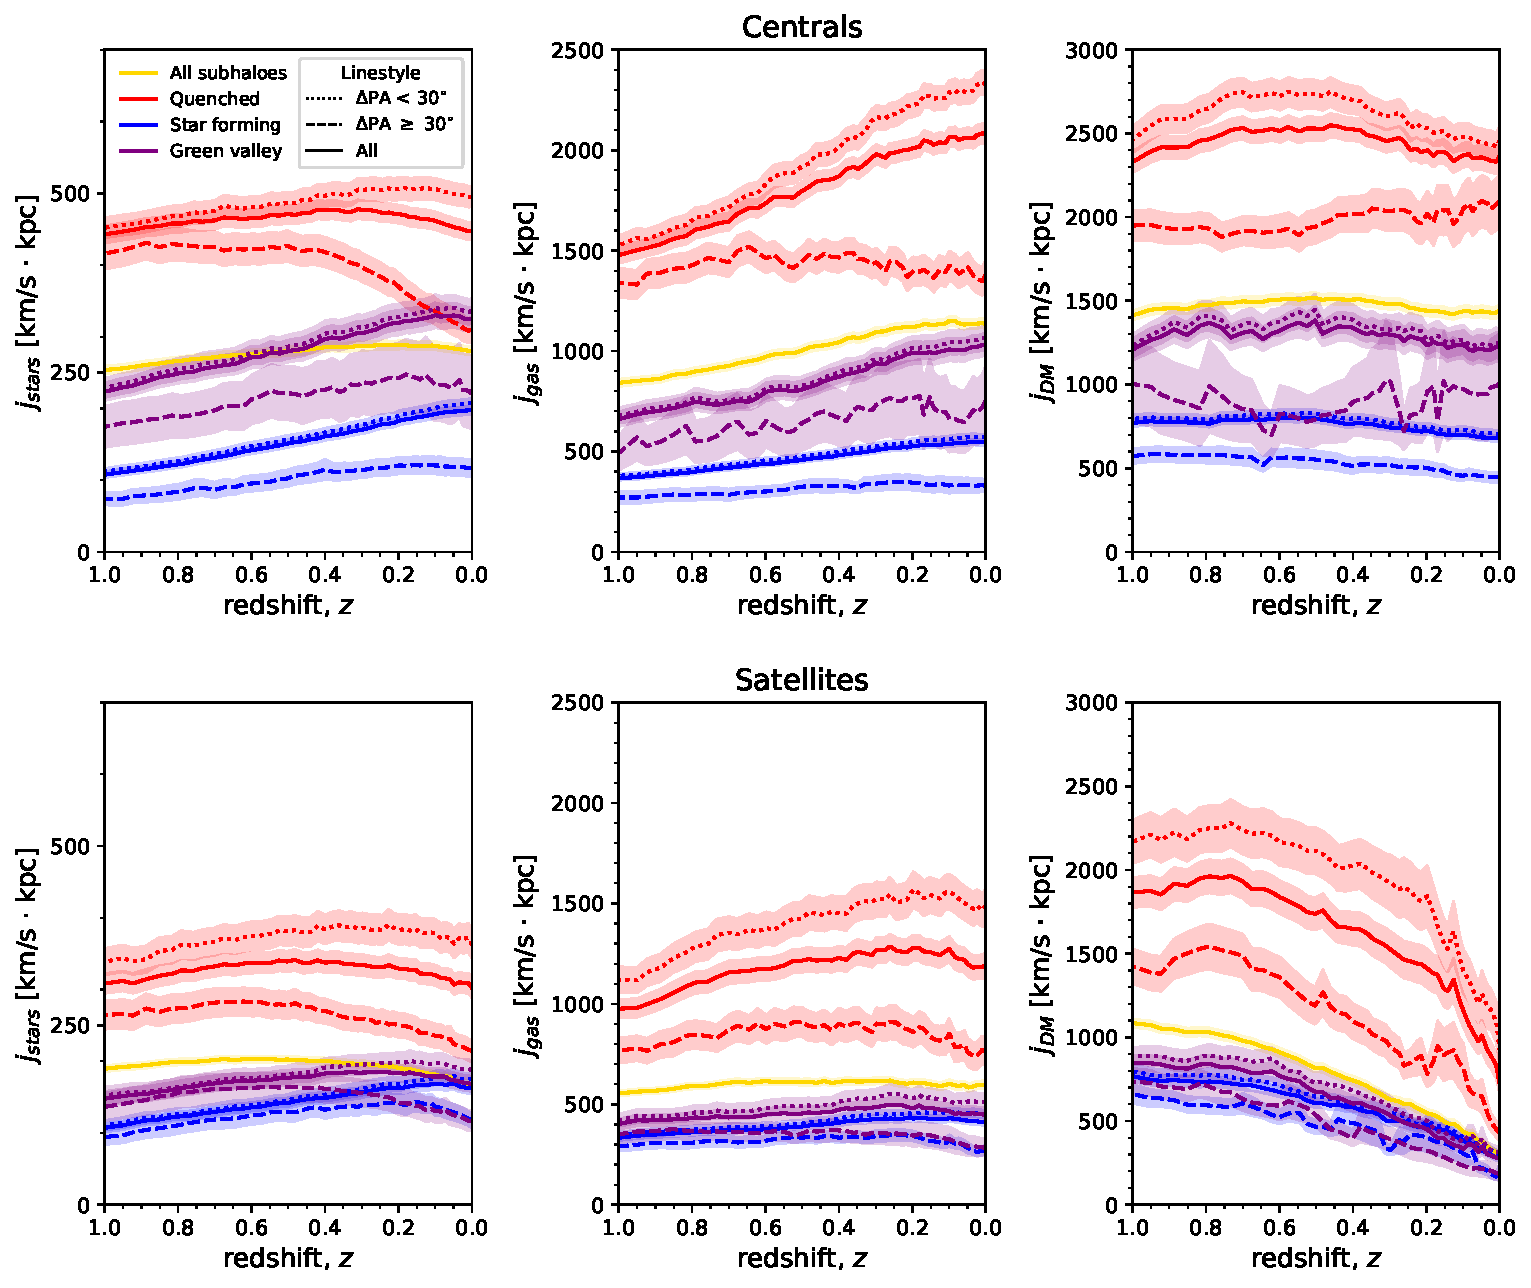
\includegraphics[width=\linewidth]{tng_results/sJ_evo_cen_sat.pdf}
    \caption{Specific angular momentum evolution from $z = 1$ for all star, gas and DM particles within the 3D radius assigned by the mock IFU observation (left to right). The evolution is taken as the median at each timestep for all galaxies of that category with errorbars showing the standard error. The top (bottom) row shows the evolution for central (satellite) galaxies. Each panel displays the evolution split into morphologies; quenched (red), green valley (purple) and star forming (blue) and also $\Delta$PA $< 30^{\circ}$ (dotted) and $> 30^{\circ}$ (dashed). Kinematically misaligned galaxies selected at $z=0$ have notably lower specific angular momentum for all of stars, gas and dark matter.}
    \label{fig:sJ_evo}
\end{figure*}

We note that particle based calculations of specific angular momentum scales with the number of particles. This results in more massive galaxies having higher $J_{i}$ and further, quenched galaxies (that are typically more massive) having higher $J_{i}$ than their later type counterparts. While there is only a small difference in-between the mass distributions of our aligned and misaligned samples (see Figure \ref{fig:TNG_mpl8_stelM}), to ensure our signal is not simply driven by mass we calculate the residuals of $J_{star}$ with respect to a typical galaxy of that mass. The residuals, $\Delta J_{star}$ are calculated by fitting a polynomial to the distribution of $J_{star}$ vs $M_{\ast}$ for the subhalos (all mock observations, regardless if $\Delta$PA is well defined) at each snapshot. $\Delta J_{star}$, is then defined as the deviation of a given galaxy away from the expectation of the fitted line at that mass. Since the trends are qualitatively consistent regardless of morphology, Figure \ref{fig:sJ_evo_residual} shows the specific angular momentum residuals for the total population. For completeness we also include the expectation for all matched subhaloes regardless of if $\Delta$PA is well defined. Misaligned galaxies ($\Delta$PA $\geq 30^{\circ}$) for both centrals and satellites show intrinsically lower $\Delta J_{star}$ indicative that it is not an effect due to mass. In addition, there is a relative evolution where $\Delta J_{stars}$ diverges from $z \sim 0.5$ so that misaligned galaxies have even lower stellar angular momentum with respect to the aligned galaxies in recent times. \red{We discuss the origin of this more recent turnoff in the section about black hole size and gas mass fraction}.

\begin{figure*}
	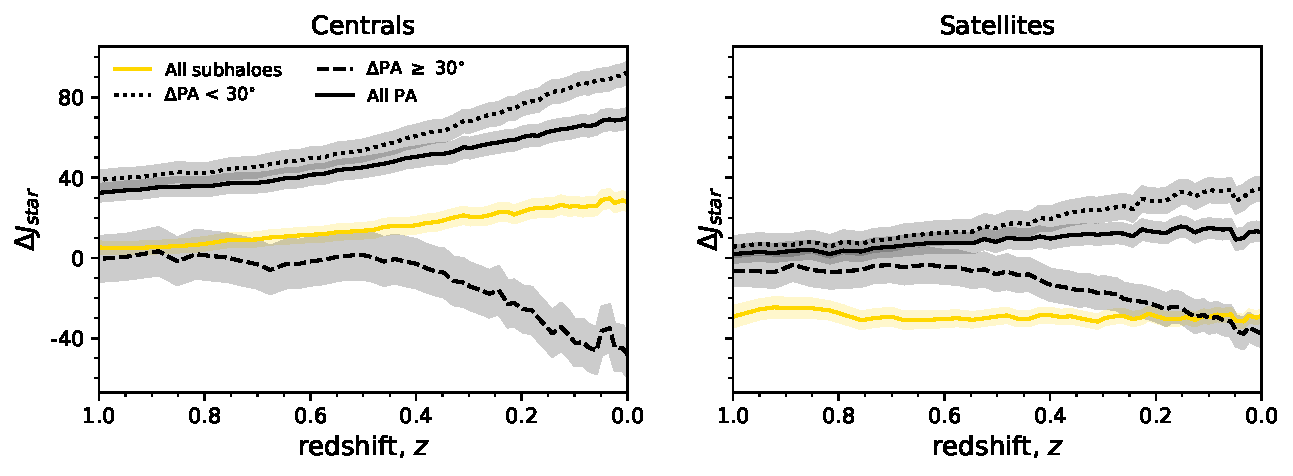
\includegraphics[width=\linewidth]{tng_results/delta_j_stars_residuals.pdf}
    \caption{The specific angular momentum residuals from $z=1$ for all star particles within the 3D radius assigned by the mock IFU observation. The residual is calculated as the deviation away from the expectation for a galaxy of that mass at each snapshot. The evolution of the residual is taken as the median at each timestep for all galaxies of that category with errorbars showing the standard error. The right (left) panel shows the evolution for central (satellite) galaxies. Each panel displays the evolution for all subhaloes (yellow), of which have a defined $\Delta$PA (black solid), aligned galaxies $\Delta$PA $< 30^{\circ}$ (black dotted) and misaligned $> 30^{\circ}$ (black dashed). We see that the difference in angular momentum between aligned and misaligned galaxies is not due to differences in mass. In addition we note a marked deviation of misaligned galaxies to even lower angular momentum in recent times. \red{update color scheme to be consistent with with ring plots.}}
    \label{fig:sJ_evo_residual}
\end{figure*}

To conclude this section we now consider the directional offsets between the angular momentum vectors of the stars, gas and dark matter. These are calculated from
\begin{equation} \label{eq:alpha}
    \alpha_{3D} = \text{arccos} \frac{\boldsymbol{J_{i}} \cdot \boldsymbol{J_{j}}}{\left| \boldsymbol{J_{i}} \right| \left| \boldsymbol{J_{j}} \right|},
\end{equation}
where $i, j$ refer to either stars, gas or dark matter. As for the magnitudes of angular momentum, the star and gas vectors are calculated within a 3D radius set to that of the IFU footprint and the dark matter vector is calculated for all particles assigned to the subhalo by subfind. Figure \ref{fig:3D_alpha_evo} shows the evolution of the 3D offsets between each of stars, gas and DM respectively. 

As expected splitting our sample on $\Delta$PA results in significantly higher $\alpha_{STARS - DM}$ at $z = 0$. In the middle panel, we see that $\alpha_{STARS - DM} \sim 50^{\circ}$ on average for galaxy mass subhaloes which is consistent with previous work \citep[e.g. see;][]{chisari+17}. For most component offsets, we see that the average $\Delta$PA misaligned population deviates away from aligned galaxies around $z \sim 0.5$. In contrast to the \textit{magnitude} of angular momentum of each component being systematically lower from at least $z = 1$ indicates the transient nature of misalignment. At any given time, the lower angular momentum haloes are simply more prone to misalignment in the baryons. This explains why ETGs are far more likely to exhibit star - gas misalignment than rotation dominated LTGs. 

\begin{figure*}
	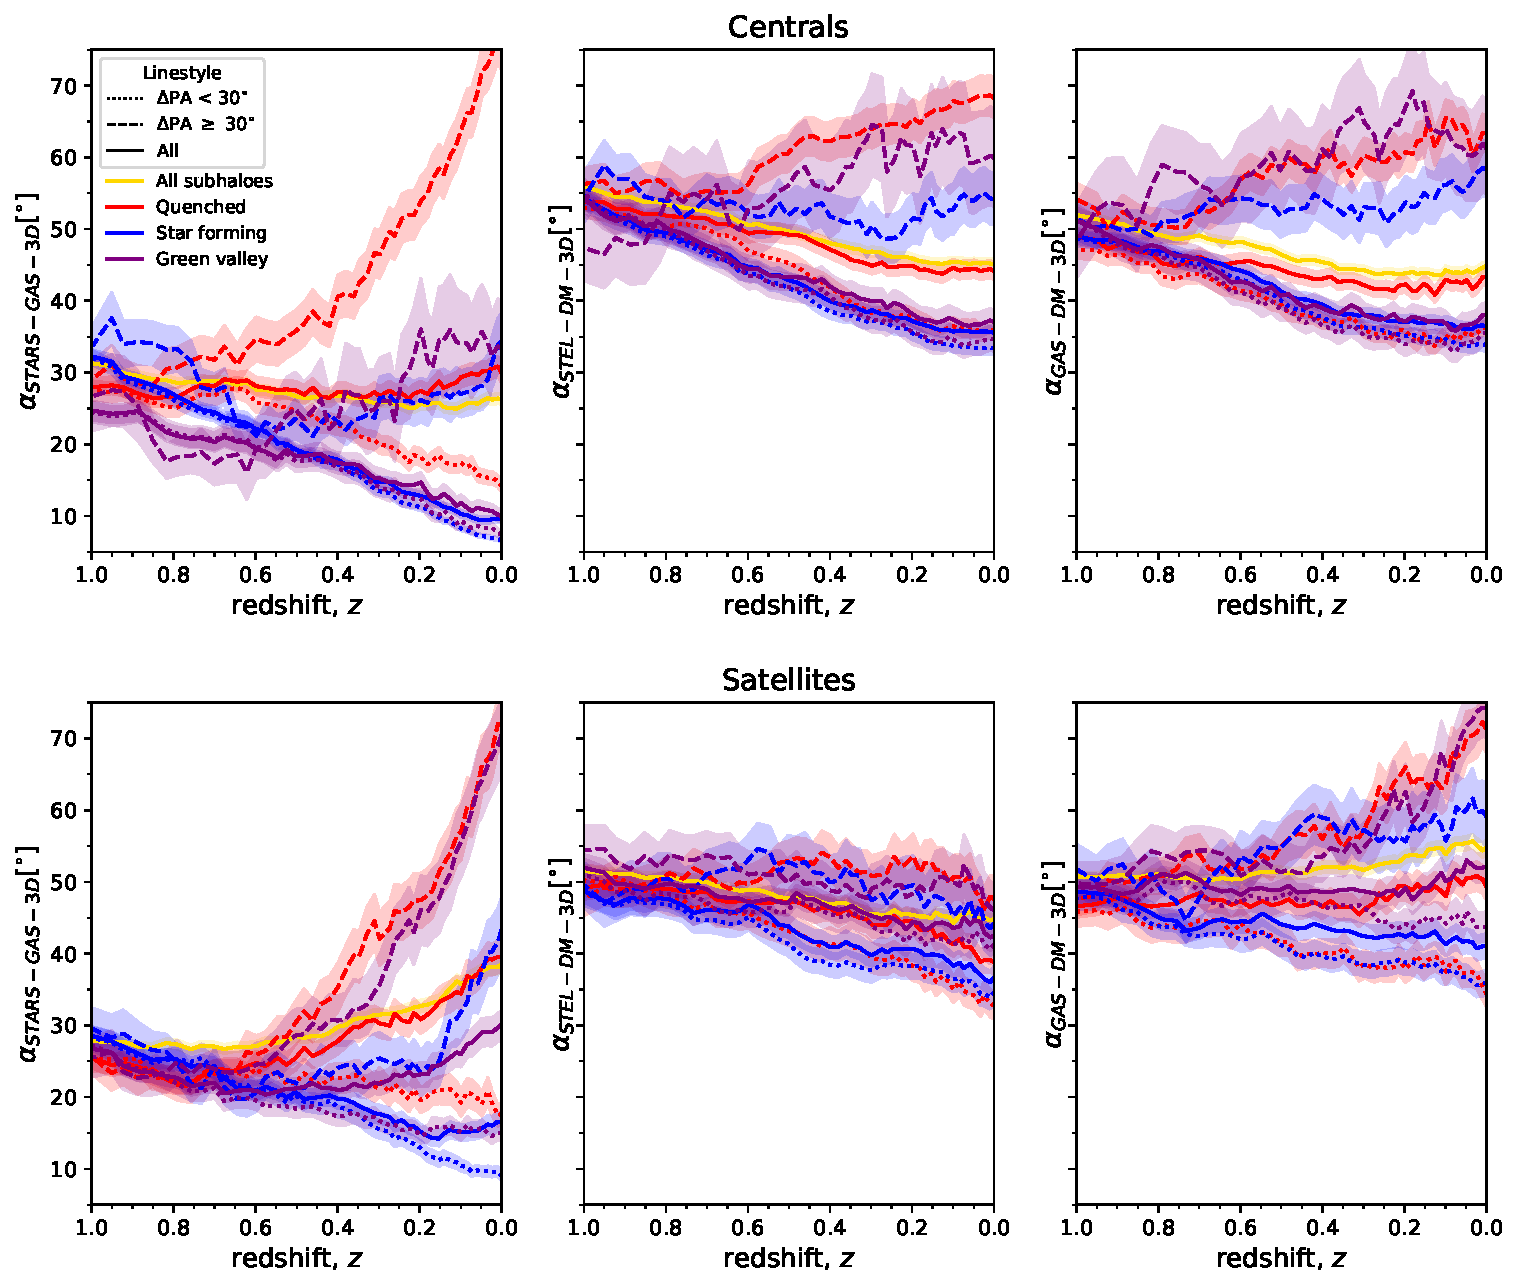
\includegraphics[width=\linewidth]{tng_results/3D_pa_evo_cen_sat.pdf}
    \caption{Evolution of the 3D offset (in degrees) between the principal spin axes of; stars and gas (left), stars and dark matter (middle) and gas and dark matter (right) from $z=1$. The evolution is taken as the median at each timestep for all galaxies of that category with errorbars showing the standard error. The top (bottom) row shows the evolution for central (satellite) galaxies. Each panel displays the evolution split into morphologies; quenched (red), green valley (purple) and star forming (blue) and also $\Delta$PA $< 30^{\circ}$ (dotted) and $\geq 30^{\circ}$ (dashed).}
    \label{fig:3D_alpha_evo}
\end{figure*}

\subsection{Assembly history}
We now consider the $z = 0$ content and assembly history of stellar mass, star forming gas and black holes for our TNG mock sample split on morphology and misalignment. Since here we make no direct comparison to observations at $z = 0$, we no longer restrict our analysis to only star or gas particles within a radius of the IFU footprint so that we can better understand the complete assembly history of the sub-population. \red{We however note that in observations that gas mass fractions are lower for misaligned objects as we see here.}

\subsubsection{Stellar mass}
In Figure \ref{fig:stel_mass_evo}, we consider the assembly time of stellar mass in our mock sample split on morphology, misalignment and group membership. We find a clear correlation with morphology for both centrals and satellites where earlier types form more of their stellar mass later. \red{why is this the case? cooling of gas - shocked gas? - gas temperature? - rate of star formation and gas accretion?}

\begin{figure*}
	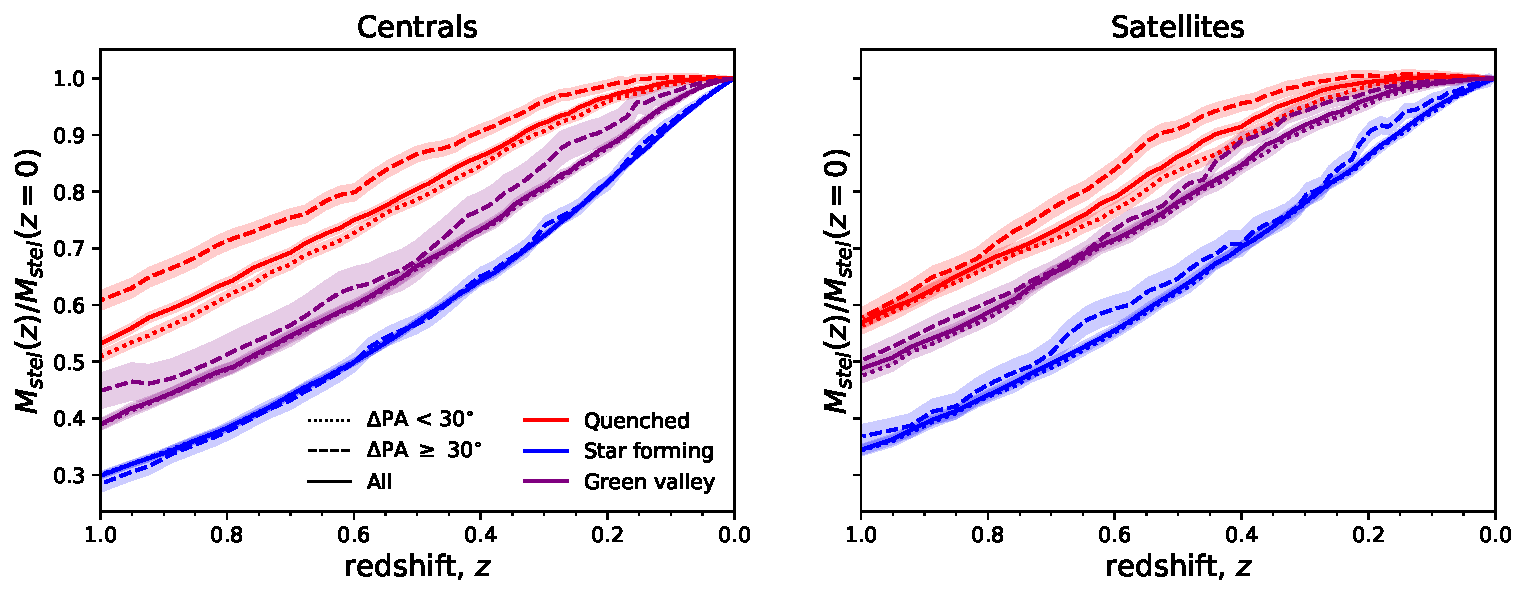
\includegraphics[width=\linewidth]{tng_results/stel_mass_timestep_norm_cen_sat.pdf}
    \caption{Evolution of the median stellar mass assembly fraction for centrals (left) and satellites (right). The stellar mass assembly fraction for each object is defined as the stellar mass at the given snapshot normalised by the stellar mass at $z = 0$. Each line shows the median and standard error for quenched (red), green valley (purple) and star forming (blue) galaxies. The solid line denotes the total population, dotted for $\Delta$PA $< 30^{\circ}$ and dashed for $\geq 30^{\circ}$.}
    \label{fig:stel_mass_evo}
\end{figure*}

\subsubsection{Black hole mass}
We now investigate the relationship between black hole mass and kinematic misalignment. In Figure \ref{fig:BH_mass}, we show the black hole mass evolution from $z = 1$ normalised by the stellar mass of the objects at each timestep. We see that for misaligned galaxies of all types, both central and satellite, have significantly higher mass black holes at least from $z \sim 0.1$ and in many cases going back much further. This is indicative that the size and hence feedback of the black hole plays as significant role in leading to misalignment. 

\begin{figure*}
	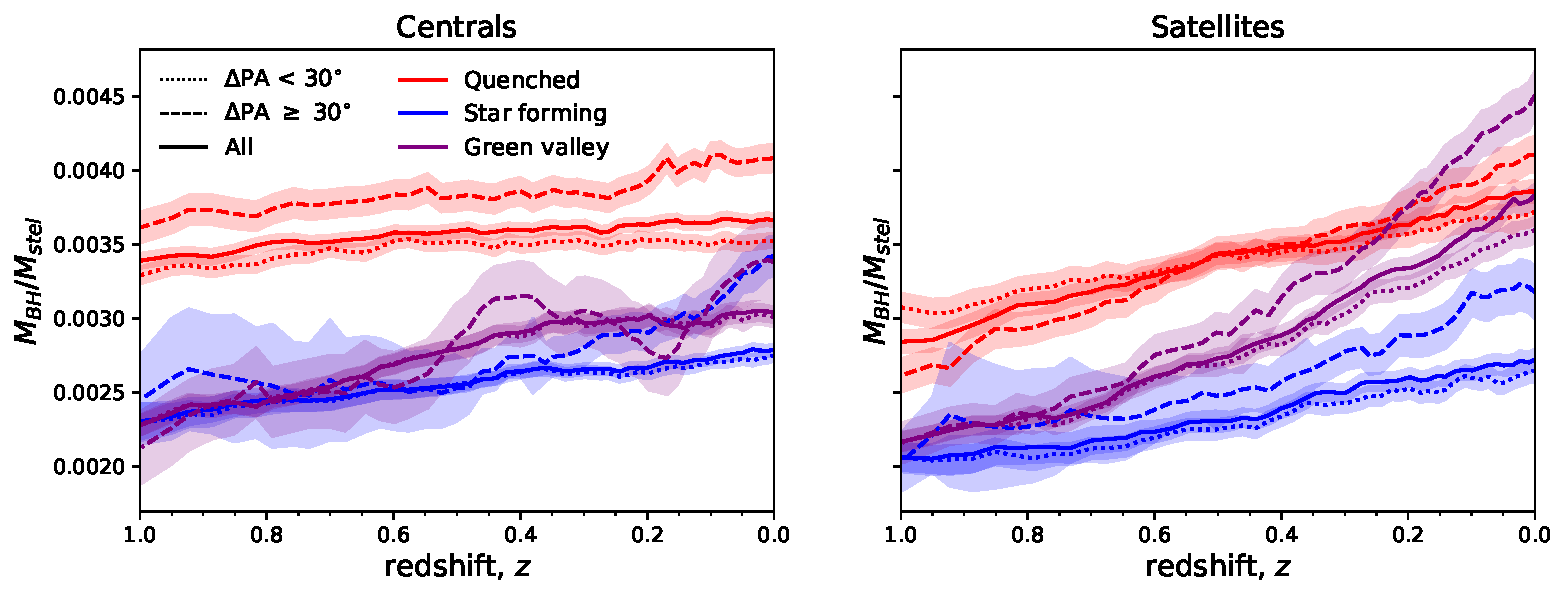
\includegraphics[width=\linewidth]{tng_results/BH_mass_timestep_norm_cen_sat.pdf}
    \caption{Evolution of the median black hole mass normalised by stellar mass from $z=1$ for centrals (left) and satellites (right). Each line shows the median and standard error for all quenched (red), green valley (purple) and star forming (blue) galaxies. The solid line denotes the total population, dotted for $\Delta$PA $< 30^{\circ}$ and dashed for $\geq 30^{\circ}$. Black hole masses are typically much larger with respect to stellar mass for misaligned galaxies.}
    \label{fig:BH_mass}
\end{figure*}

\subsection{Gas mass and metallicity}

\begin{figure*}
	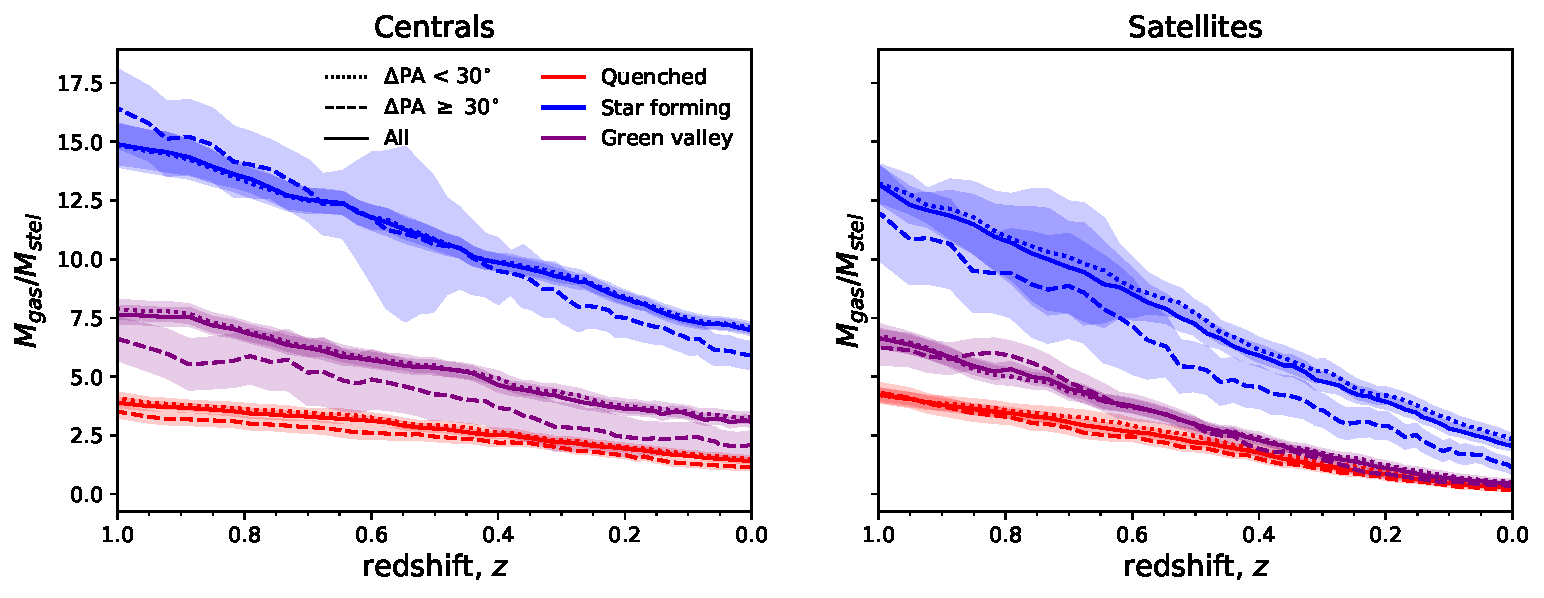
\includegraphics[width=\linewidth]{tng_results/gas_mass_timestep_norm_cen_sat.pdf}
    \caption{Evolution of the median gas mass normalised by stellar mass from $z=1$ for centrals (left) and satellites (right). Each line shows the median and standard error for quenched (red), green valley (purple) and star forming (blue) galaxies. The solid line denotes the total population, dotted for $\Delta$PA $< 30^{\circ}$ and dashed for $\geq 30^{\circ}$. Gas masses are typically much smaller with respect to stellar mass for misaligned galaxies.}
    \label{fig:gas_mass}
\end{figure*}

\begin{figure*}
	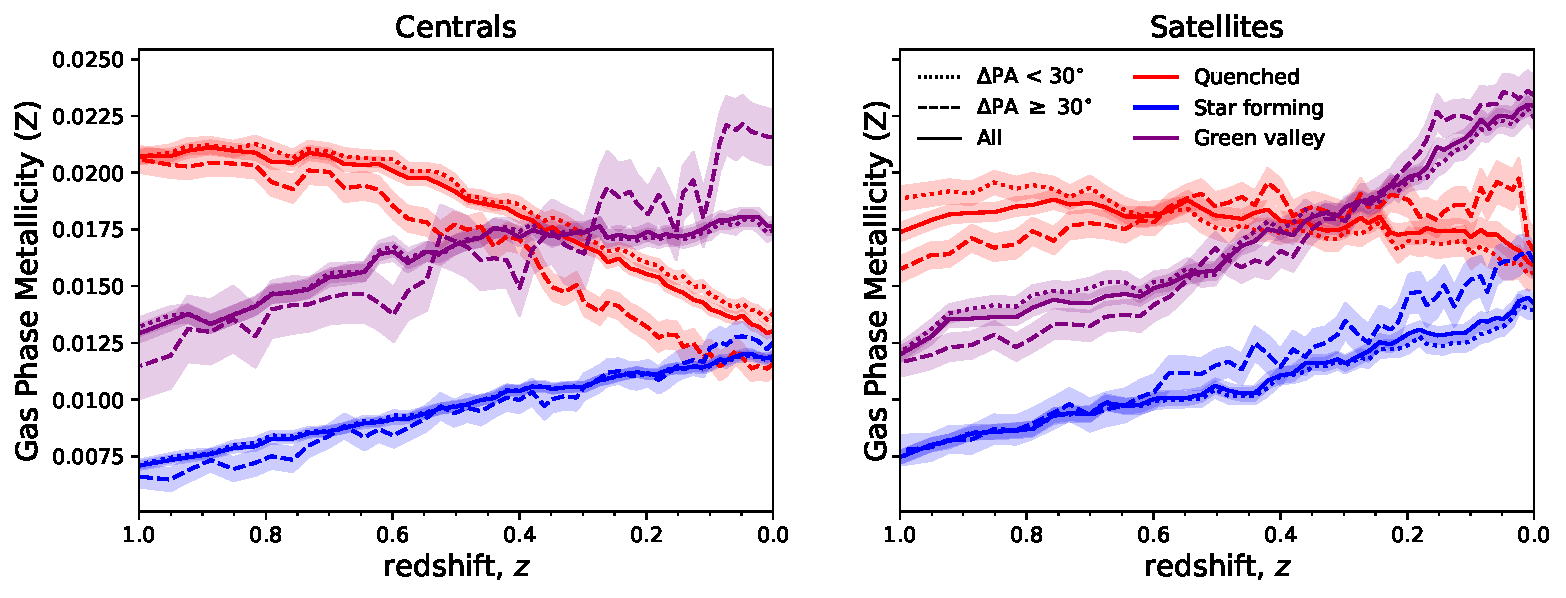
\includegraphics[width=\linewidth]{tng_results/gas_metallicity_nonorm_cen_sat.pdf}
    \caption{Evolution of the un-normalised gas phase metallicity from $z=1$ for centrals (left) and satellites (right). Each line shows the median and standard error for quenched (red), green valley (purple) and star forming (blue) galaxies. The solid line denotes the total population, dotted for $\Delta$PA $< 30^{\circ}$ and dashed for $\geq 30^{\circ}$.}
    \label{fig:gas_metallicity}
\end{figure*}

\begin{figure*}
	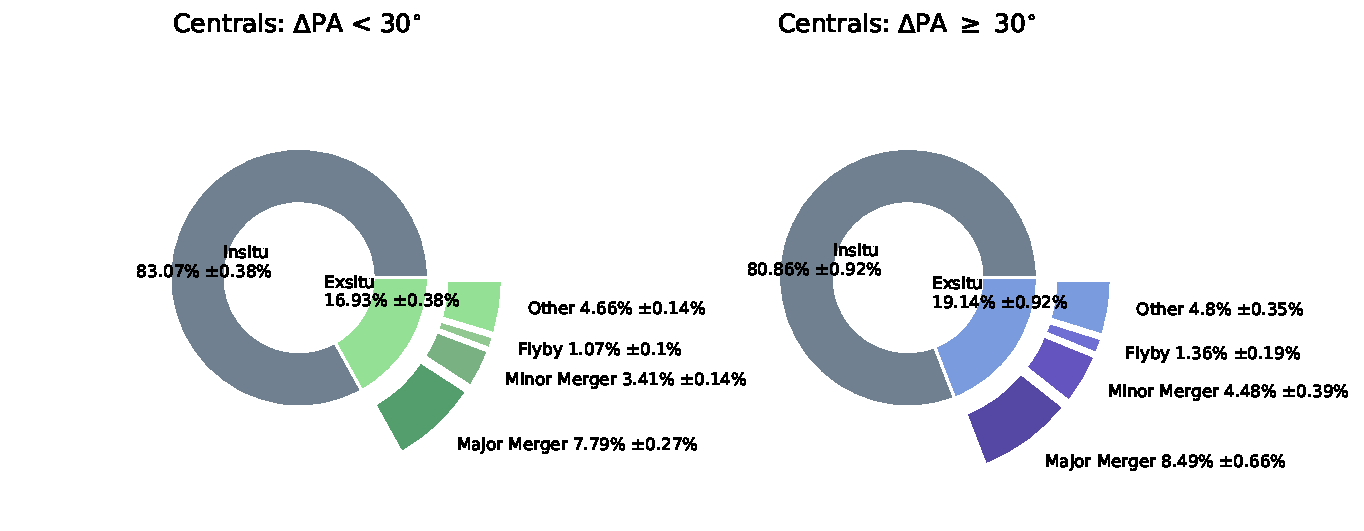
\includegraphics[width=\linewidth]{tng_results/gas_donut_centrals_PA_split.pdf}
    \caption{Breakdown of stellar mass origination for kinematically aligned centrals (left; $\Delta$PA < 30$^{\circ}$) and misaligned centrals (right; $\Delta$PA $\geq$ 30$^{\circ}$). Each sector shows the average fraction of stellar mass originating from a given process for the population. The inner ring describes the in-situ/ ex-situ gas fractions with the outer ring displaying the fractions for the ex-situ category. Misaligned central galaxies acquire a larger fraction of stellar mass from ex-situ processes.}
    \label{fig:cen_gas_donut}
\end{figure*}

\begin{figure*}
	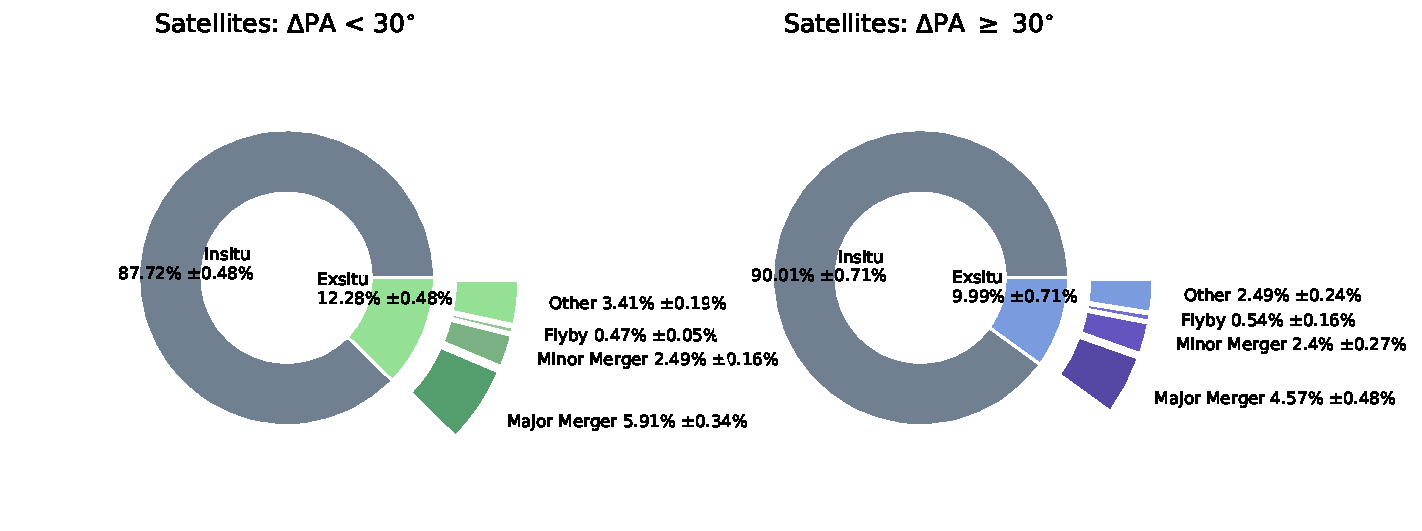
\includegraphics[width=\linewidth]{tng_results/gas_donut_satellites_PA_split.pdf}
    \caption{Same as Figure \ref{fig:cen_gas_donut} but for satellite galaxies. Misaligned satellite galaxies acquire a lesser fraction of stellar mass from ex-situ processes.}
    \label{fig:sat_gas_donut}
\end{figure*}

\subsection{Merger history}

\begin{figure}
	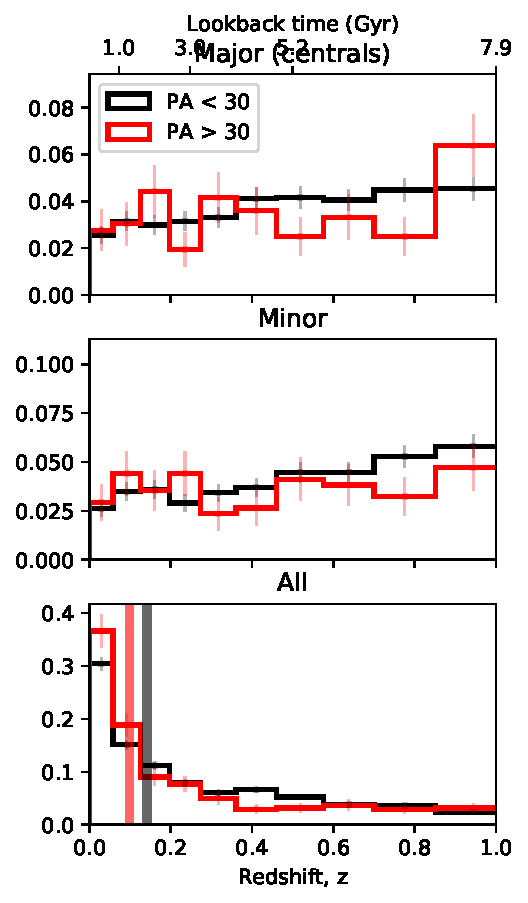
\includegraphics[width=\linewidth]{tng_results/time_since_last_merger_centrals_PA_split.pdf}
    \caption{Time since last (major, minor, all mass ratios) mergers for central galaxies.}
    \label{fig:last_merger_cen}
\end{figure}

\begin{figure}
	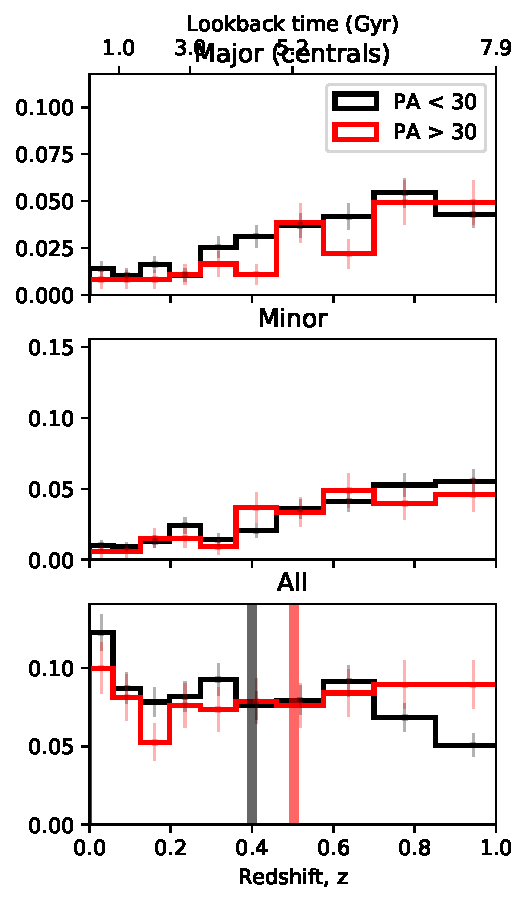
\includegraphics[width=\linewidth]{tng_results/time_since_last_merger_satellites_PA_split.pdf}
    \caption{Time since last (major, minor, all mass ratios) mergers for satellite galaxies.}
    \label{fig:last_merger_sat}
\end{figure}

\section{Discussion}

We note the close relationship of our findings of our mock TNG sample with respect to the work of \citet{starkenburg+19}. They investigate the origin of star-gas counter-rotation (i.e $ > 90^{\circ}$) using individual case studies of low mass galaxies (i.e $2 \times 10^{9} < M_{\ast} < 5 \times 10^{10}$) in the original Illustris simulation \red{check this description}. Despite extending the mass range and only considering overall trends for aligned and misaligned galaxies split at $\Delta$PA$= 30^{\circ}$ in the updated physics prescriptions of TNG, we still find the same qualitative trends of lower angular momentum, lower gas mass and larger black holes for our misaligned samples. Black hole feedback clearly holds an important role in disrupting the angular momentum content of galaxies leading to the future increased likelihood of star-gas misalignment in the prescriptions of both Illustris and TNG. 

The relative importance of black hole activity in creating misaligned \textit{real} galaxies with respect to internal processes is yet to be fully determined. \citet{chen2016} and \citet{jin2016} construct a picture of misaligned galaxies acquiring new gas from gas-rich dwarfs which disrupt angular momentum leading to increased inflow and boosted star formation in central regions. \textit{Could the same inflows then lead to triggering of AGN or is it the feedback from the black hole creating the misalignment in the first place?}. \citet{roy2018} determine that around 5-10\% of quiescent galaxies in MaNGA have large scale AGN-driven winds characterised by high velocity bi-symmetric flows in H$\alpha$ leading to a distinct gas-star misalignments of $\sim 90^{\circ}$. While this appears to be a special galaxy population of fast rotating ETGs, this demonstrates that the role of feedback is intrinsically linked to the gas misalignment in both simulation and observation to some degree. The transient nature of both AGN and kinematic misalignment make causality a difficult prospect, however, we leave the correlation between AGN and the prevalence of kinematic misalignment the focus of future work. 

We also note TNGs ability to not only recreate a reasonable distribution of $\Delta$PAs with respect to the MaNGA sample (see Fig \ref{fig:total_pa_dist}) once accounting for variances in mass between the $\Delta$PA defined samples in MaNGA and TNG (\red{because the misaligned TNG sample is slightly more massive which may mean more galaxies are likely to be misaligned}) but also reproducing the strong trends with morphology found in observations (see Fig \ref{fig:group_morph_TNG} in comparison to \ref{fig:group_morph_PA}). 

\bibliographystyle{mnras}
\bibliography{biblio.bib}

%%%%%%%%%%%%%%%%%%%%%%%%%%%%%%%%%%%%%%%%%%%%%%%%%%

%%%%%%%%%%%%%%%%% APPENDICES %%%%%%%%%%%%%%%%%%%%%
\section*{Acknowledgements}

\appendix

\section{Characterisation of mock sample} \label{sec:mock_appendix}
This section characterises the mock MaNGA sample created in TNG. Figure \ref{fig:TNG_mpl8_stelM}, shows the stellar mass distributions of the aligned and misaligned samples in both MPL-8 and TNG. Since the mock sample is matched for all MPL-8 galaxies it is natural that there would be some variation in the stellar mass distributions of the mock and observational $\Delta$PA samples. The overall distribution matches well, however, with the TNG sample having a clear boost of galaxies at the high mass end of the distribution with respect to the equivalent in MPL-8.

\begin{figure}
	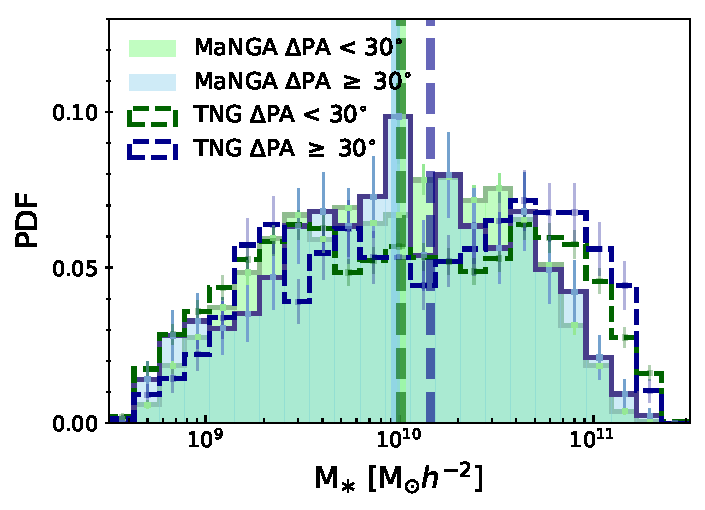
\includegraphics[width=\linewidth]{tng_appendix/delPA_split_stelM_tng_comparison.pdf}
    \caption{Probability density distributions of stellar mass, $(M_{\ast}/M_{\odot})$ for aligned galaxies ($\Delta$PA < 30$^{\circ}$, green) and misaligned galaxies ($\Delta$PA > 30$^{\circ}$, red) defined in MPL-8 (solid lines) and TNG (dashed). The overall distributions are a reasonable match between mocks and observations, with a noted preference for $\Delta$PA defined galaxies at the very high mass end for TNG.}
    \label{fig:TNG_mpl8_stelM}
\end{figure}

Figure \ref{fig:group_morph_TNG}, shows the $\Delta$PA distribution for the TNG sample split into centrals and satellites. \red{Describe the morphological classification.} Comparing to the observational sample in Figure \ref{fig:group_morph_PA}, the morphological trends remain qualitatively the same with quenched/ETGs (star forming/LTGs) more likely to be misaligned (aligned). 

\begin{figure*}
	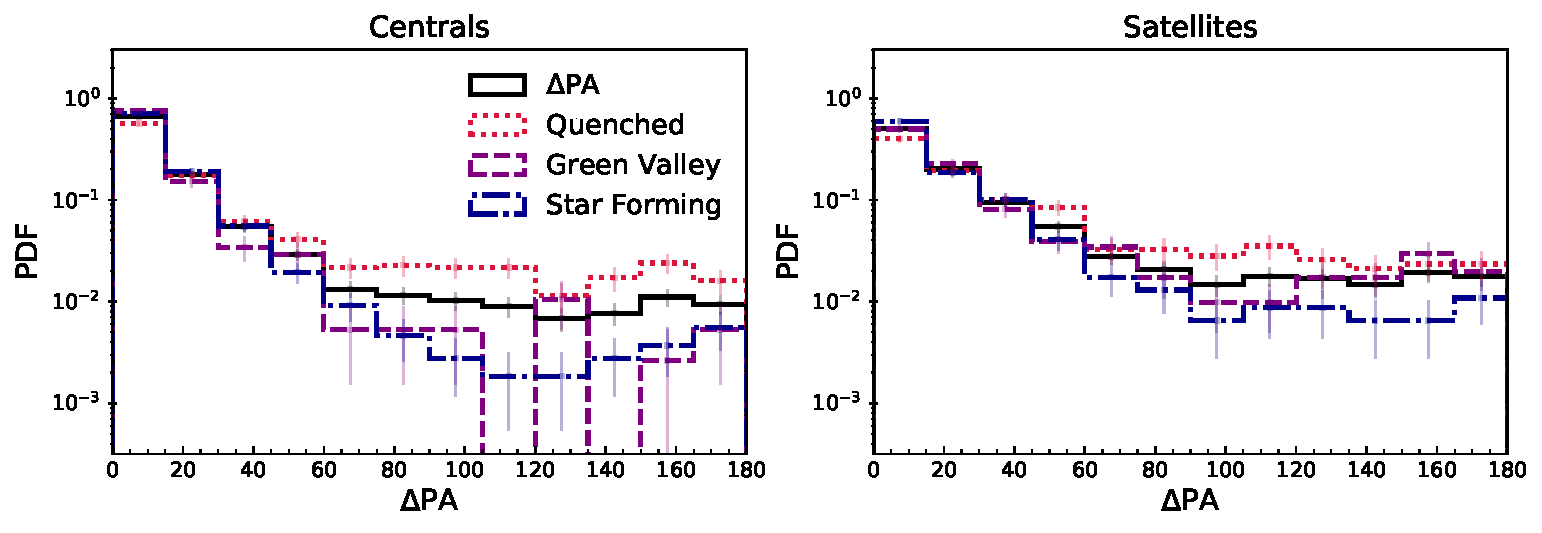
\includegraphics[width=\linewidth]{tng_appendix/TNG_delPA_sfms_group.pdf}
    \caption{Same as Figure \ref{fig:group_morph_PA}, however for the mock TNG sample. Morphology in this instance is categorised by the deviation of the galaxy's star formation away from the main sequence of galaxies in the whole of TNG.}
    \label{fig:group_morph_TNG}
\end{figure*}

\section{PA vs absolute offset} \label{sec:PA_test}
A key assumption of this work is the ability for the projected $\Delta$PA to be a reliable estimator of the actual 3D offset between star and gas rotation axes. Figure \ref{fig:PA_residual} shows the distributions of the difference between $\Delta$PA and the 2D and 3D offsets between the angular momentum principal axes of stars and gas. See equation \ref{eq:alpha} for calculation of the 3D offset; the 2D equivalent is simply a projection of this onto the XY plane. $\Delta$PA is a reasonable measure of the true 3D offset which can be modelled as a Gaussian centred on 0$^{\circ}$ with a standard deviation of 17.6$^{\circ}$ (green dotted line). The deviation of the 2D projection from the true 3D offset (black line) has a standard deviation of 13$^{\circ}$, demonstrating that the variation is both due to projection and the noise associated with observations.

\red{discuss different particle selection.}

\begin{figure}
	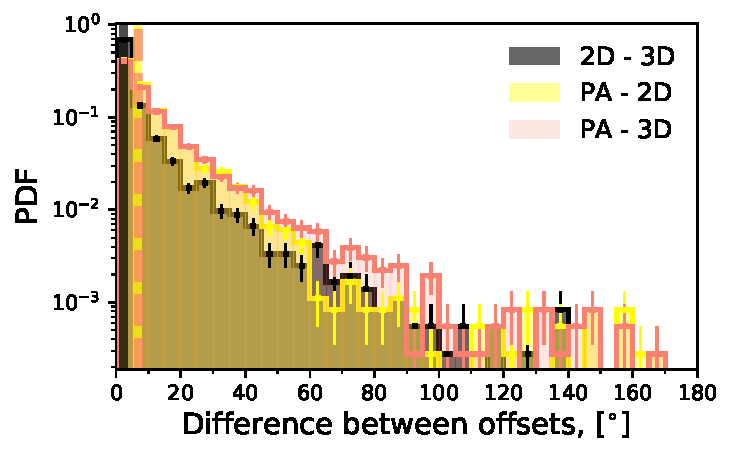
\includegraphics[width=\linewidth]{tng_appendix/PA_alpha_resid_hist.pdf}
    \caption{Probability density distribution of the difference between various measures of the star-gas rotational angle offset. The difference between the 3D angular momentum vectors and projection in 2D is shown (black), $\Delta$PA and 2D (yellow) and $\Delta$PA and 3D (blue).}
    \label{fig:PA_residual}
\end{figure}
%%%%%%%%%%%%%%%%%%%%%%%%%%%%%%%%%%%%%%%%%%%%%%%%%%


% Don't change these lines
\bsp	% typesetting comment
\label{lastpage}
\end{document}

% End of mnras_template.tex